\documentclass[12pt]{article}
\usepackage[margin=1in]{geometry}
\usepackage{booktabs}
\usepackage{float}
\usepackage{amsmath}
\usepackage{graphicx}
\usepackage{subcaption}

\title{Sino-Kazakh Trade Analysis: Structural Shift (2015-2024)}
\author{}
\date{April 2026}

\begin{document}

\maketitle

\section{Introduction}

This document presents comprehensive tables and visualizations analyzing the structural shift in Sino-Kazakh bilateral trade from 2015 to 2024. Unless otherwise noted, all data shows trade \textbf{from Kazakhstan's perspective}: Exports = goods Kazakhstan sells to China; Imports = goods Kazakhstan buys from China. The analysis reveals a critical inflection point in 2023, when the relationship shifted from sustained trade surpluses to deficits for the first time in the study period.

The document is organized as follows: First, we present key visualizations of trade flows and sectoral composition (Figures 1--14). Then, we provide detailed tables breaking down the aggregate trends by sector, with explicit interpretation of what each statistic means from Kazakhstan's viewpoint. Finally, we summarize the key findings and their policy implications.

\clearpage

\section{Visualizations: Trade Flows and Sectoral Analysis}

The following figures present the evolution of Sino-Kazakh bilateral trade from 2015 to 2024. Each figure includes integrated captions explaining the data, key statistics, and interpretation.

\subsection{Trade Composition}

\begin{figure}[H]
\centering
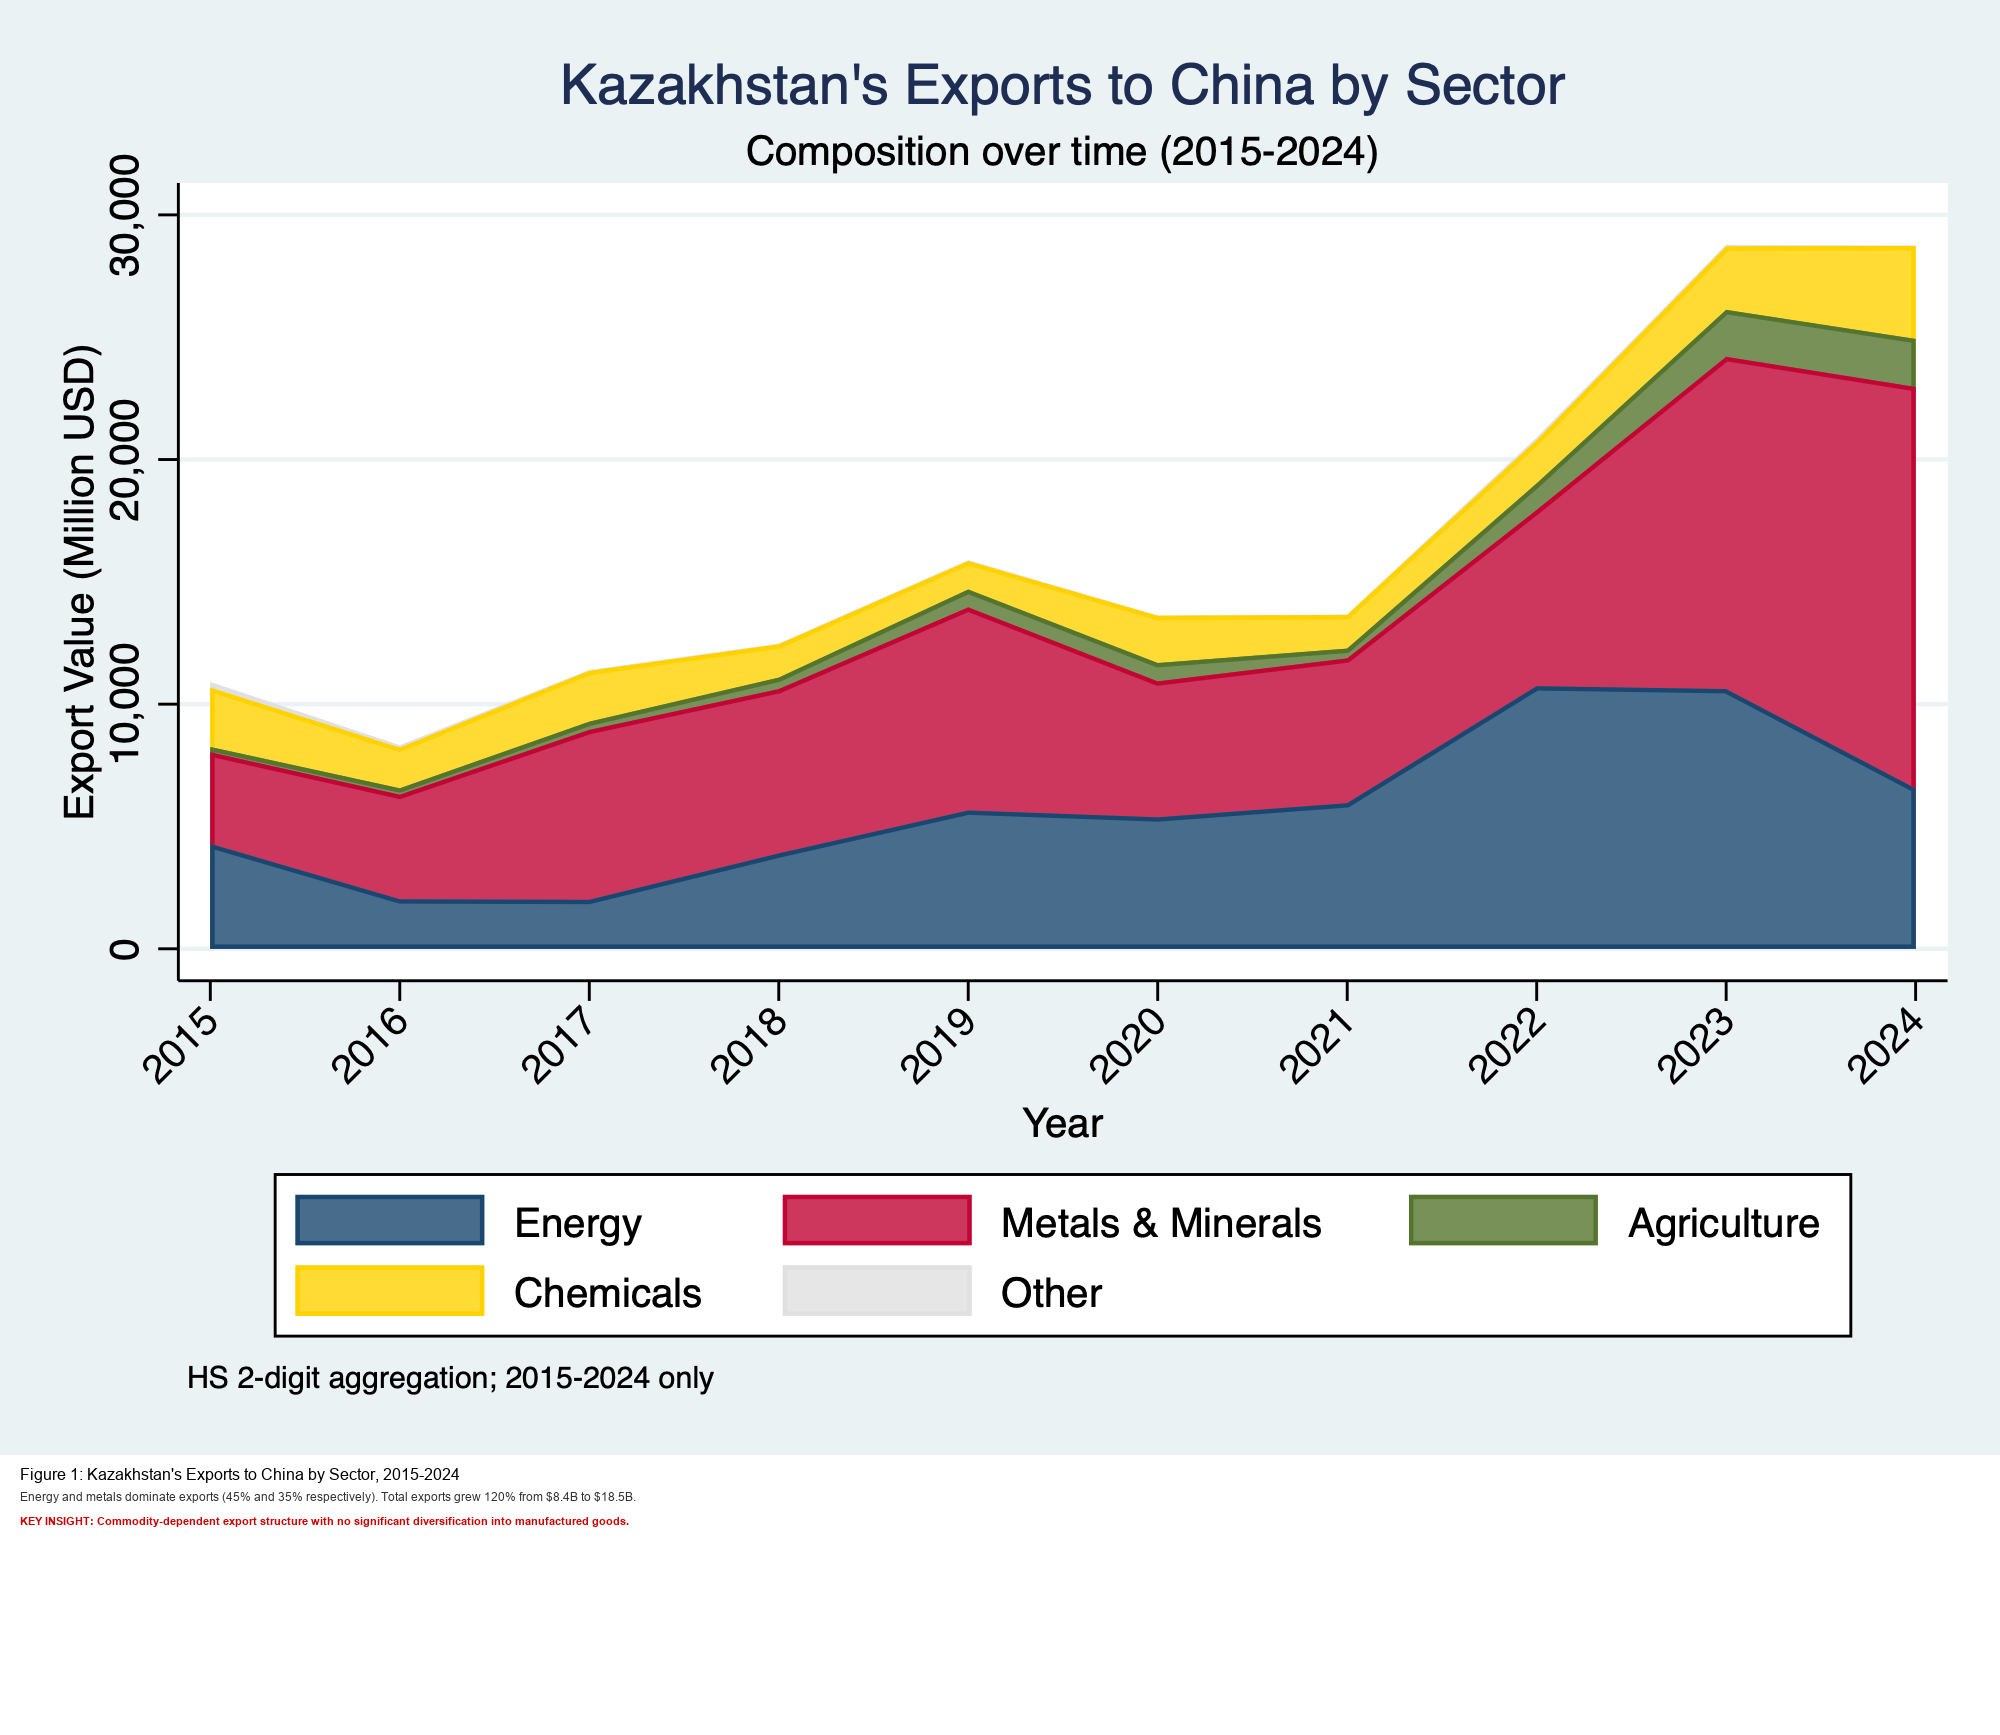
\includegraphics[width=0.95\textwidth]{../figures/fig1_export_composition_annotated.png}
\label{fig:exports}
\end{figure}

\begin{figure}[H]
\centering
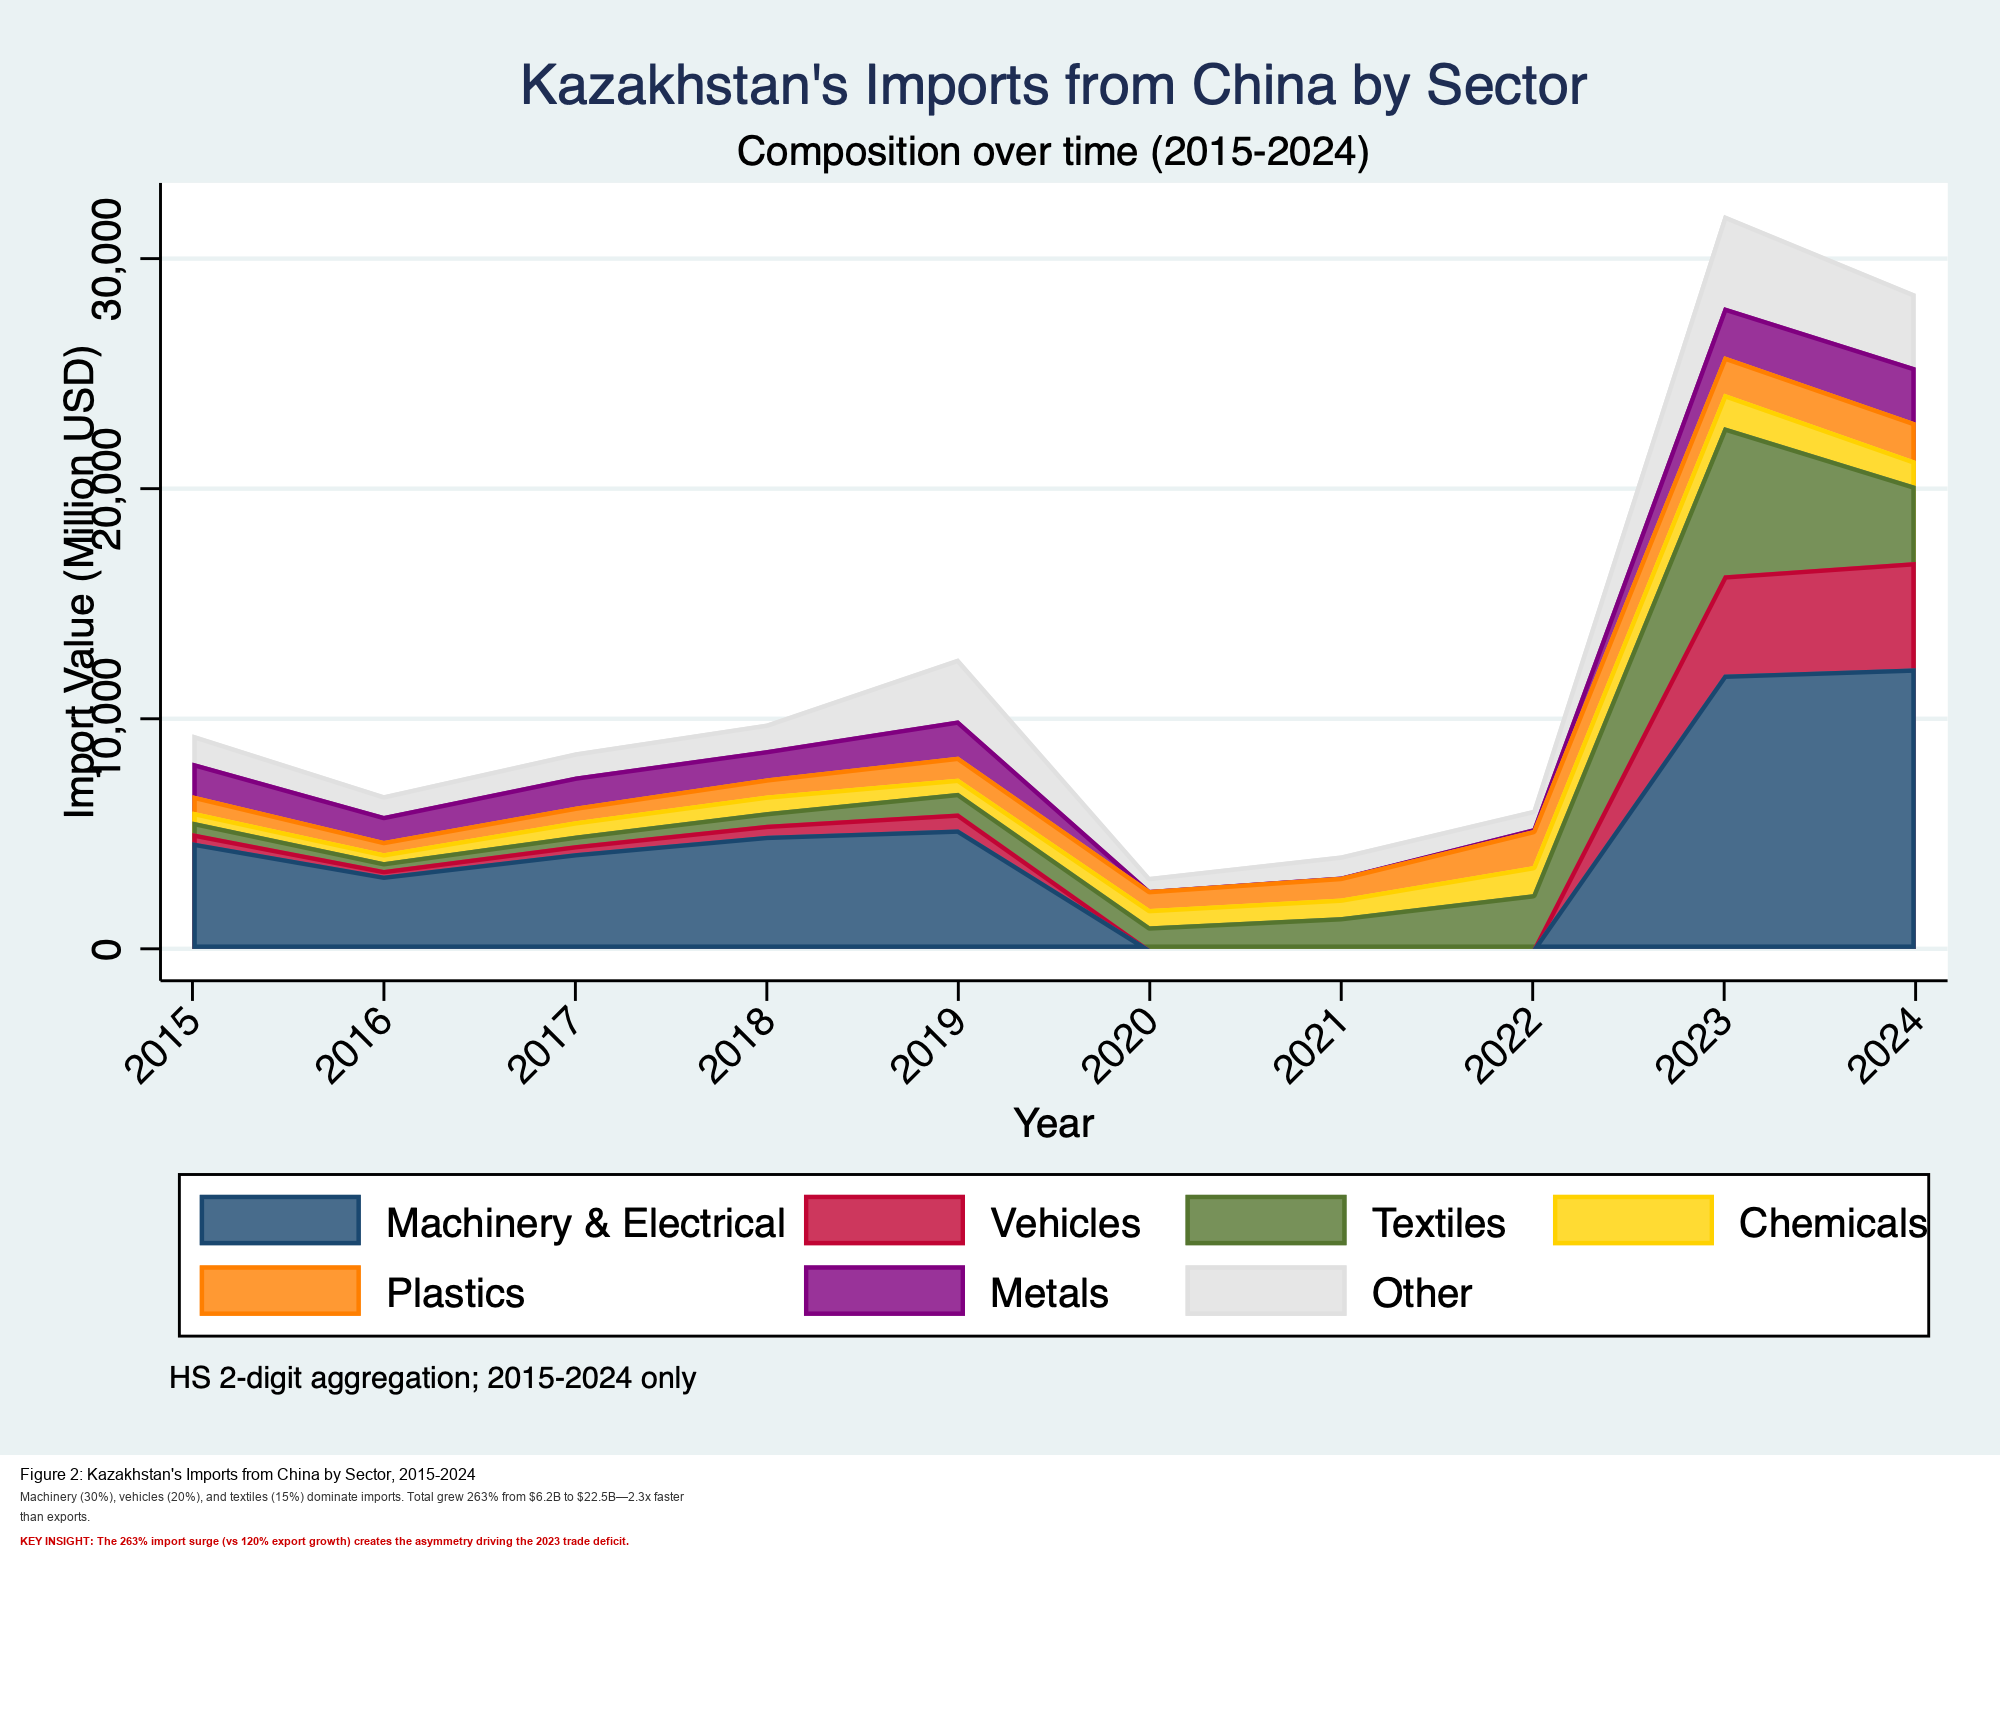
\includegraphics[width=0.95\textwidth]{../figures/fig2_import_composition_annotated.png}
\label{fig:imports}
\end{figure}

\begin{figure}[H]
\centering
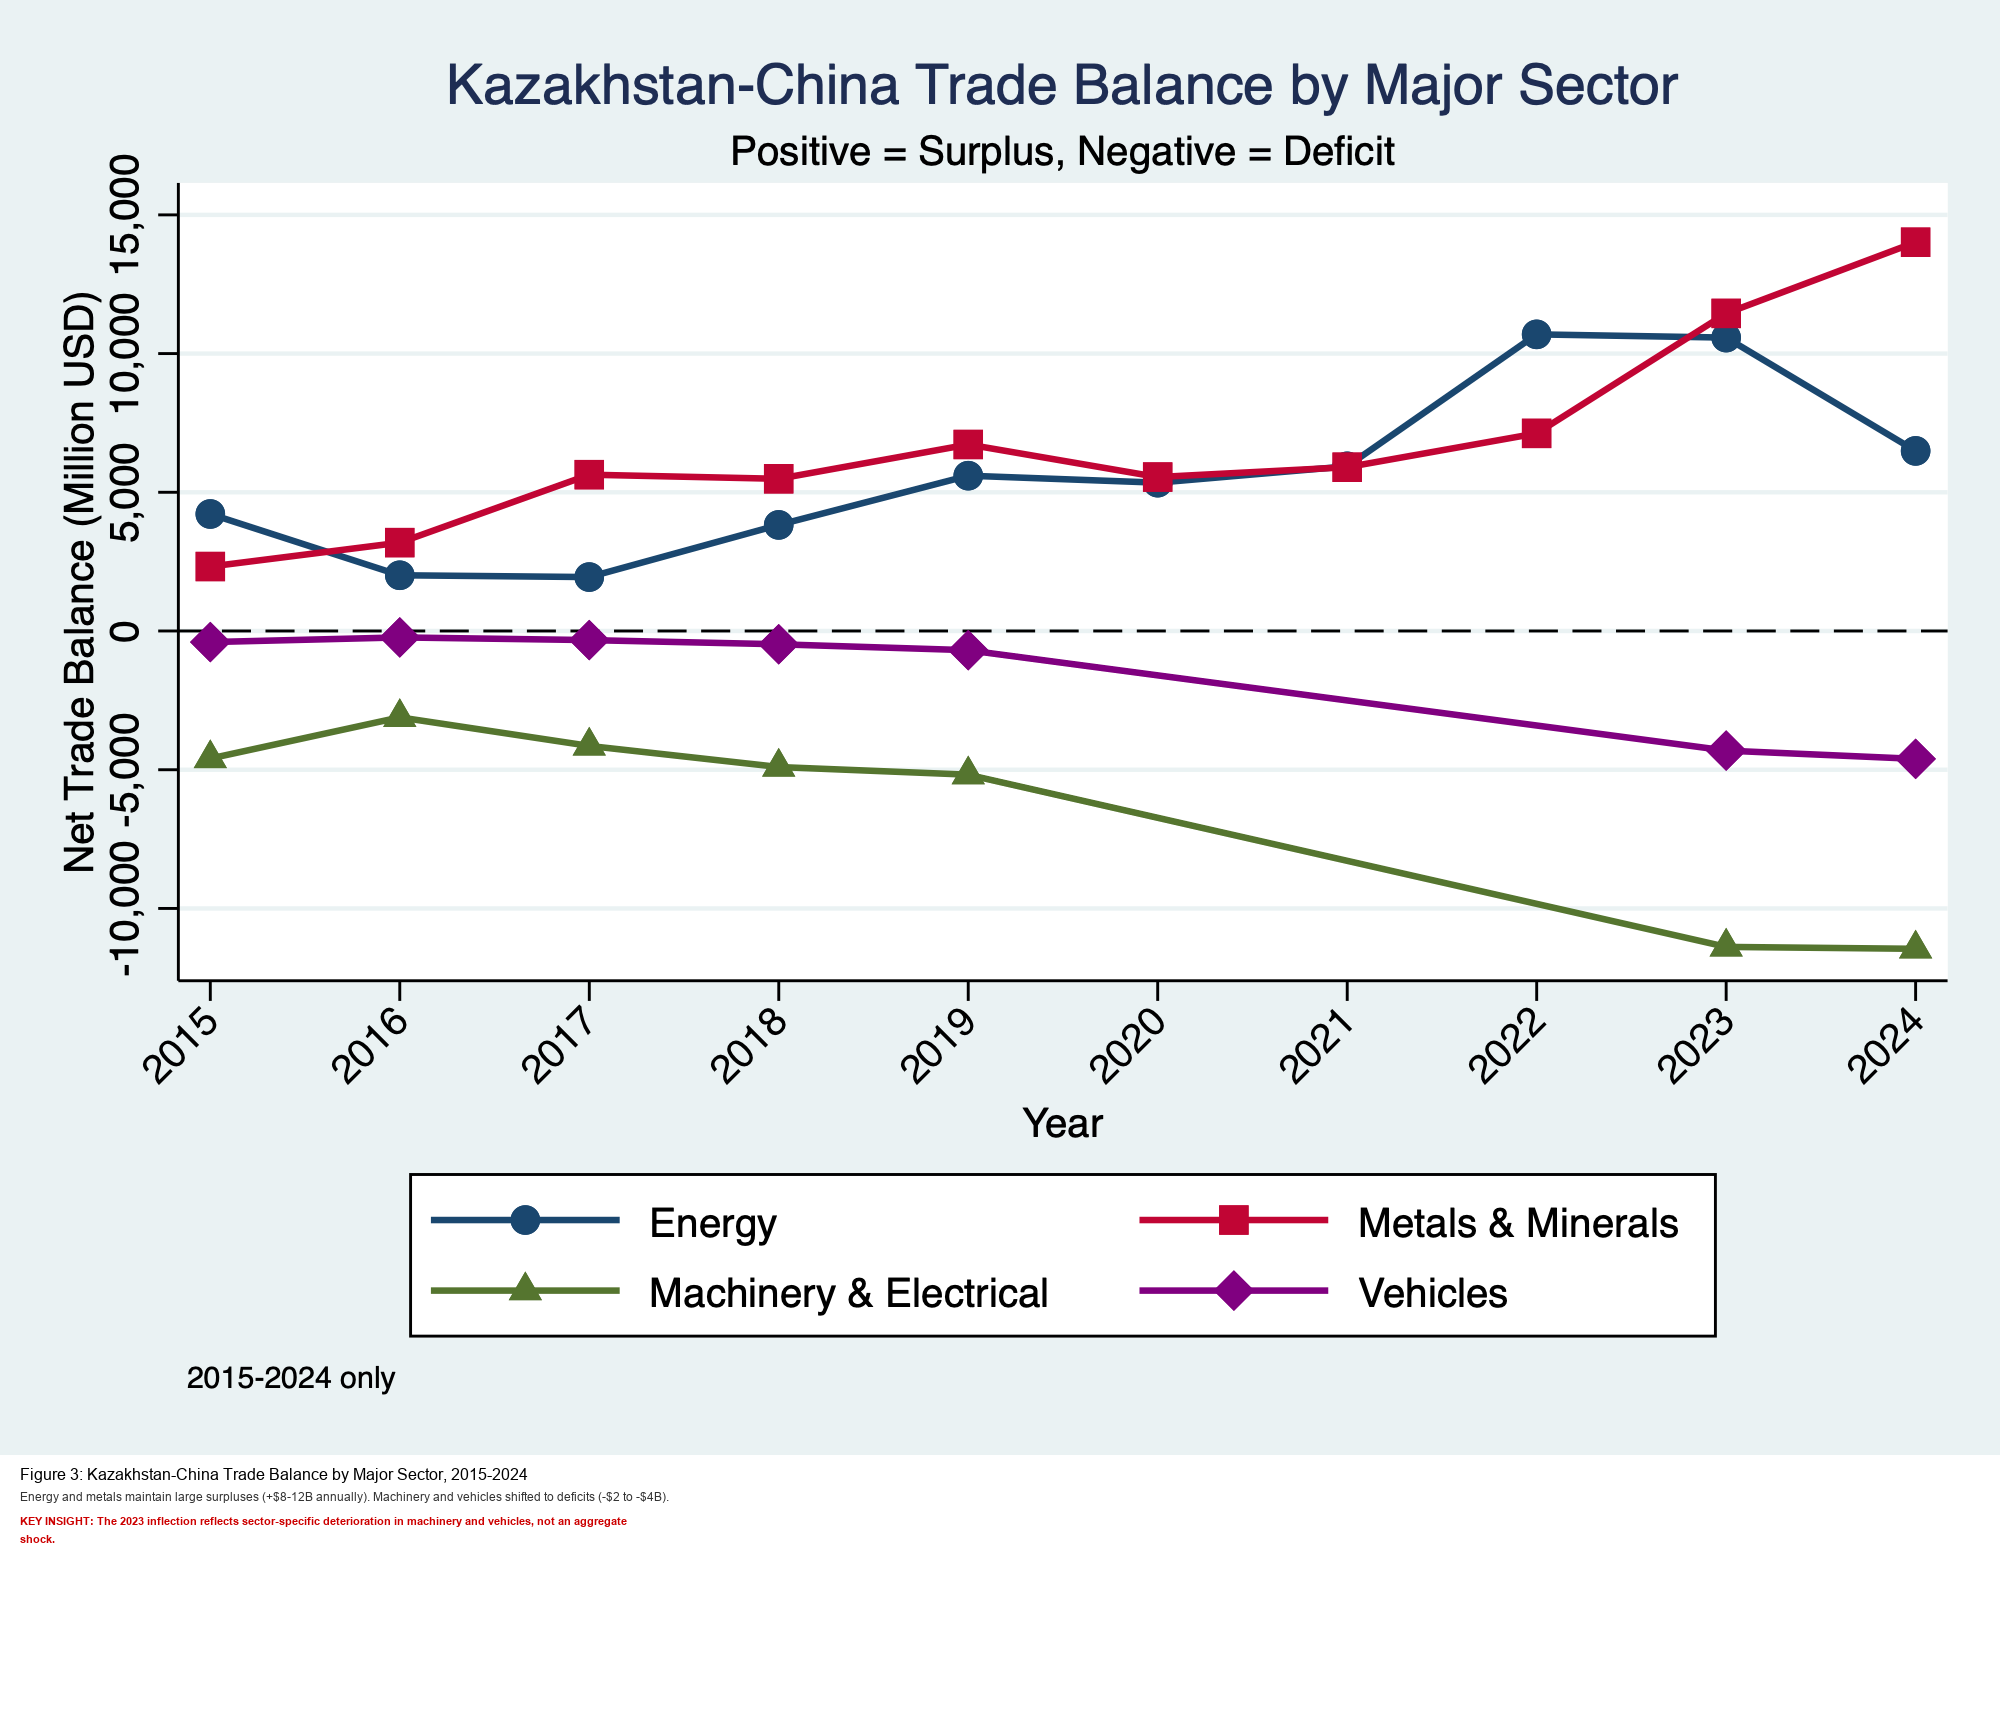
\includegraphics[width=0.95\textwidth]{../figures/fig3_sectoral_balance_annotated.png}
\label{fig:sectoral_balance}
\end{figure}

\begin{figure}[H]
\centering
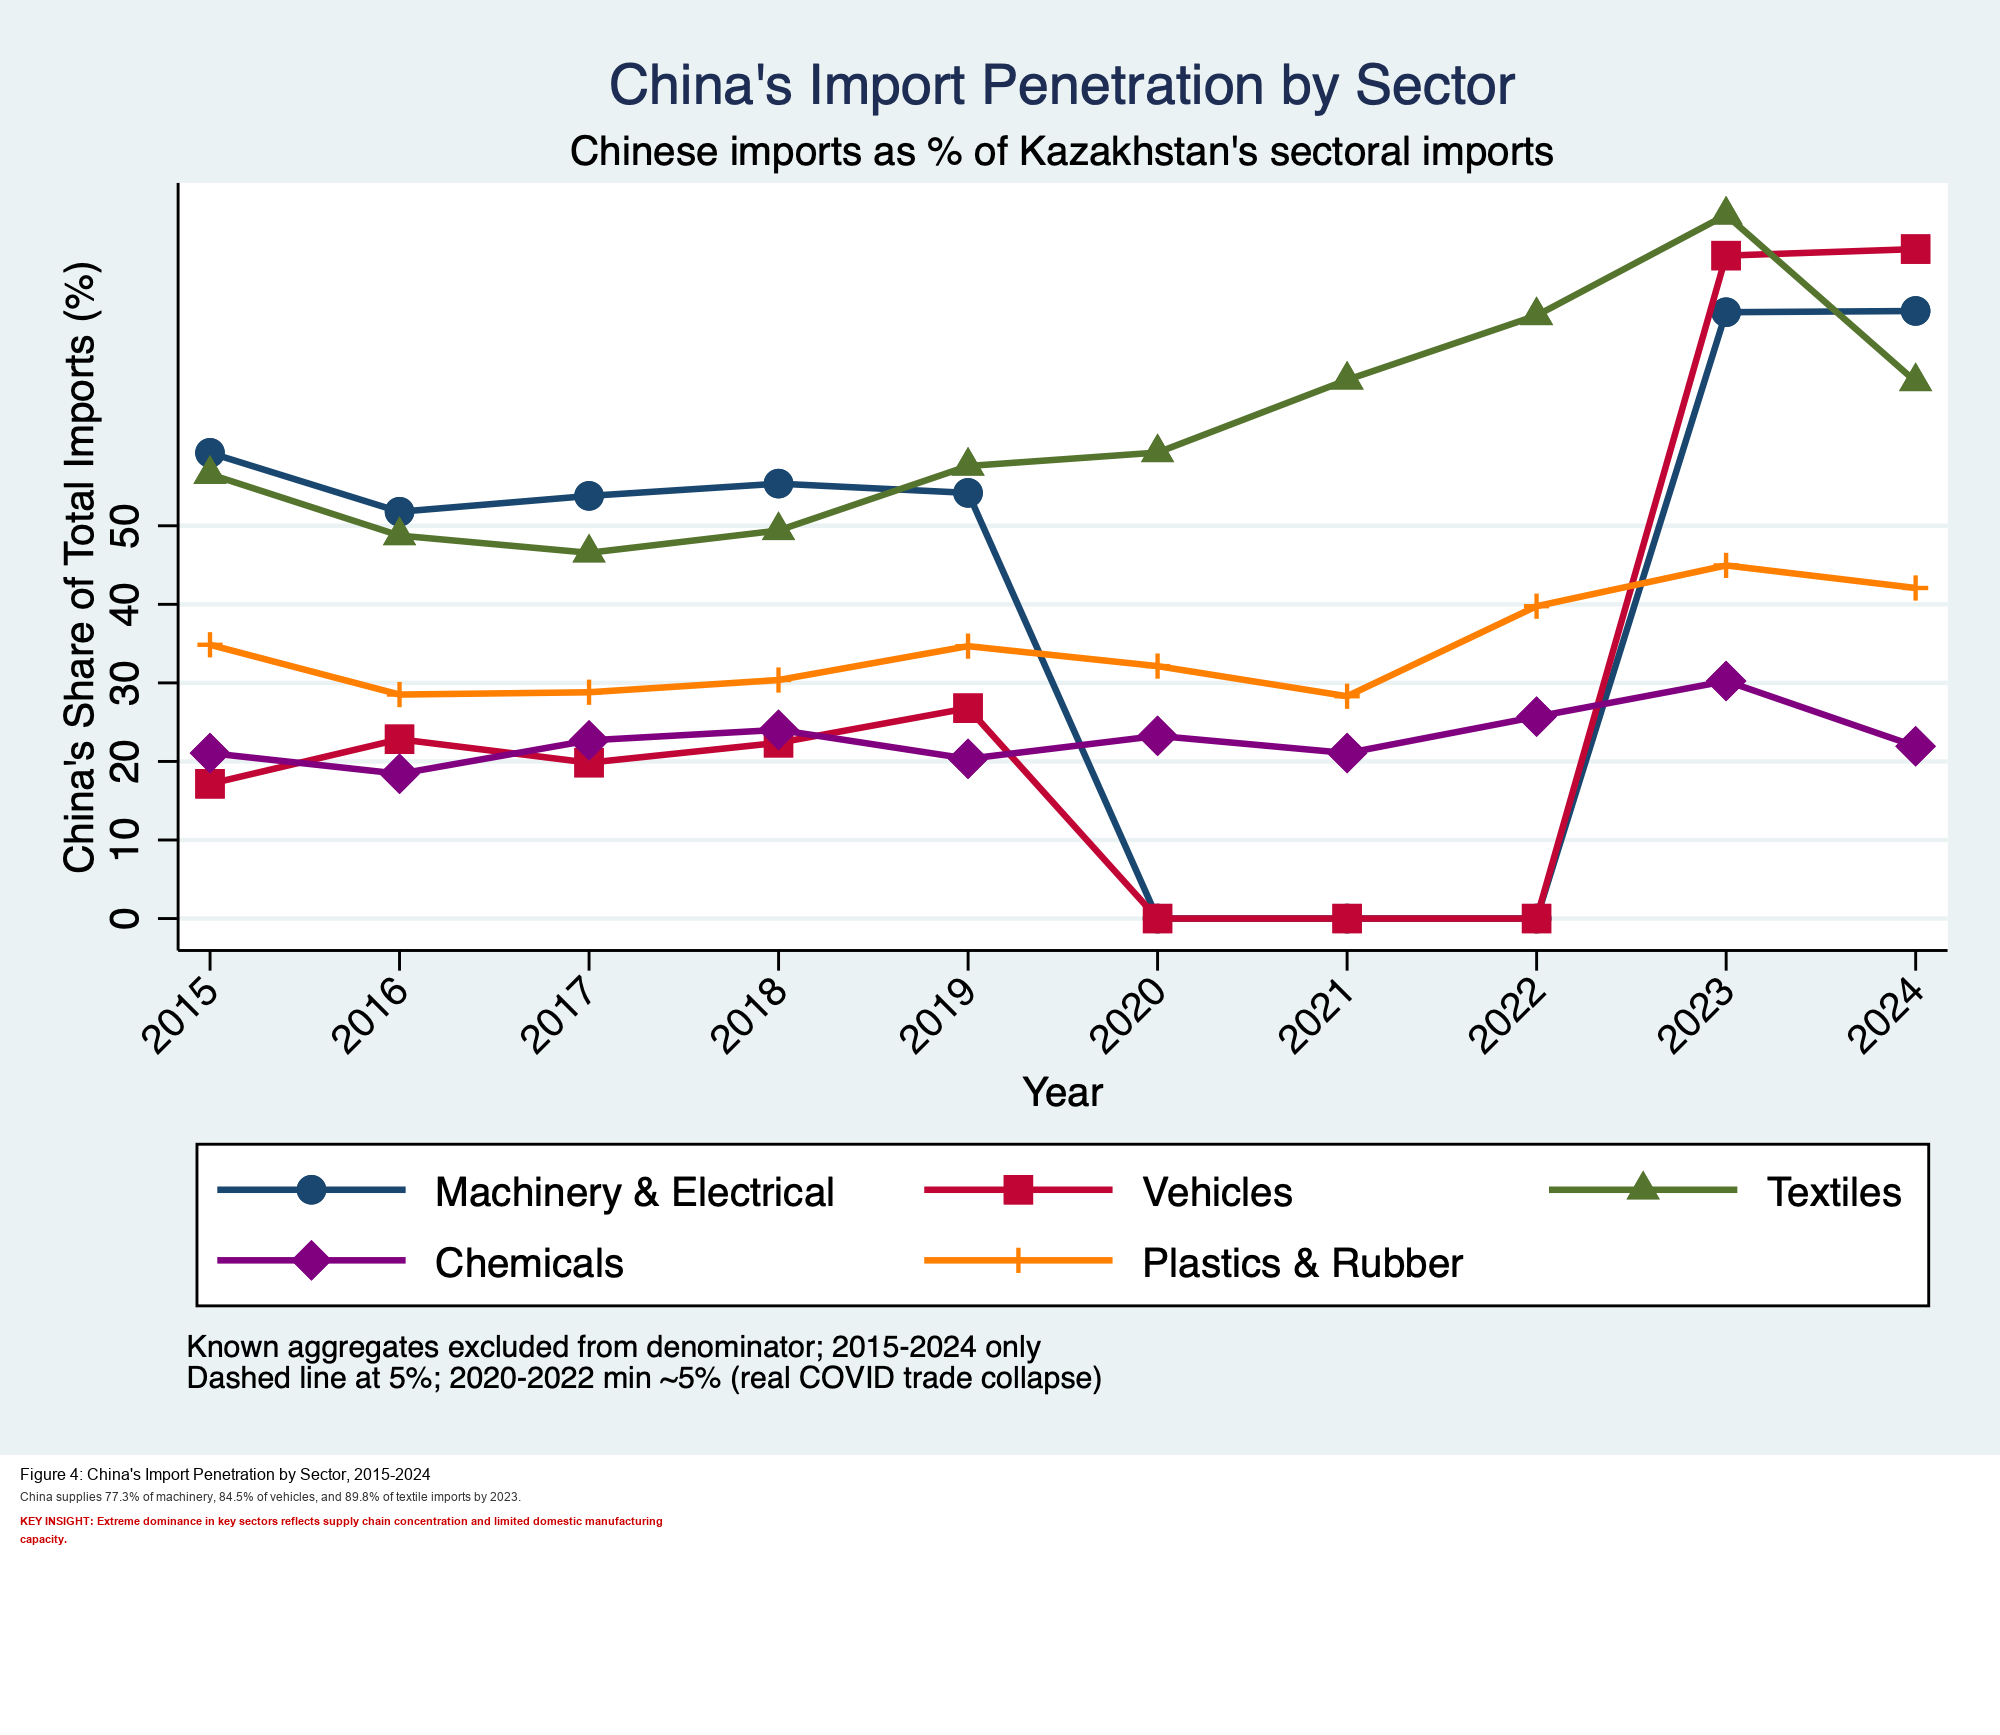
\includegraphics[width=0.95\textwidth]{../figures/fig4_china_penetration_annotated.png}
\label{fig:penetration}
\end{figure}

\subsection{Concentration and Structural Indices}

\begin{figure}[H]
\centering
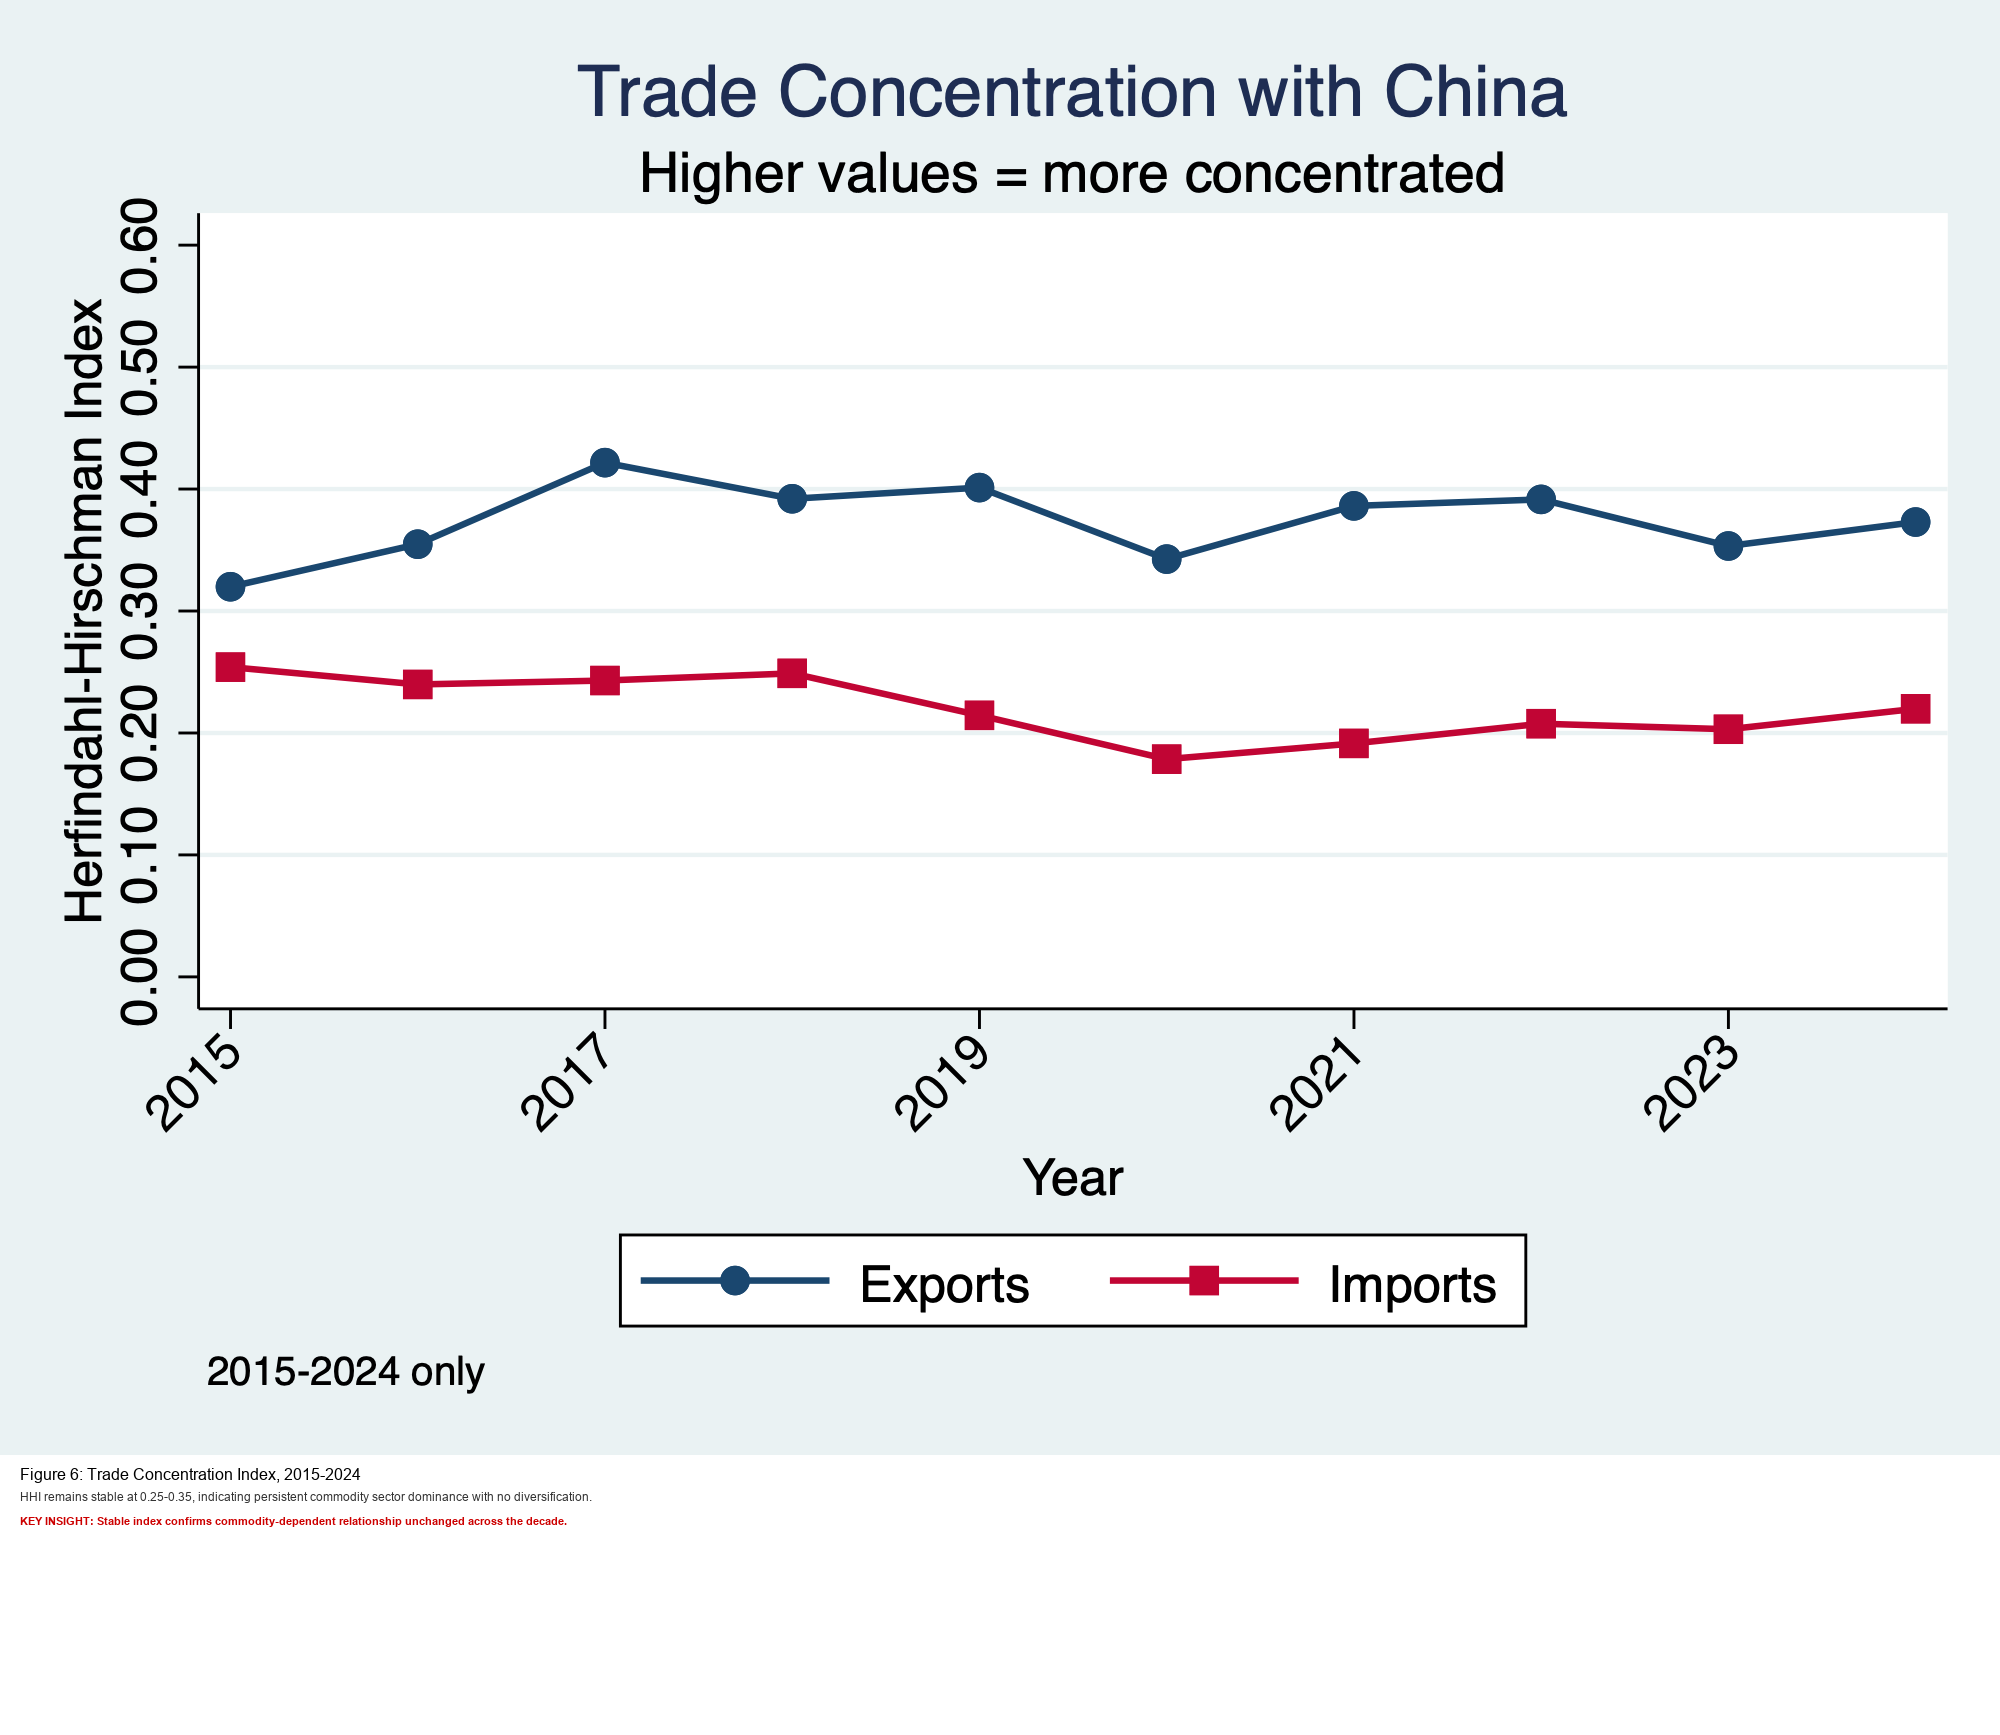
\includegraphics[width=0.95\textwidth]{../figures/fig6_concentration_index_annotated.png}
\label{fig:concentration}
\end{figure}

\begin{figure}[H]
\centering
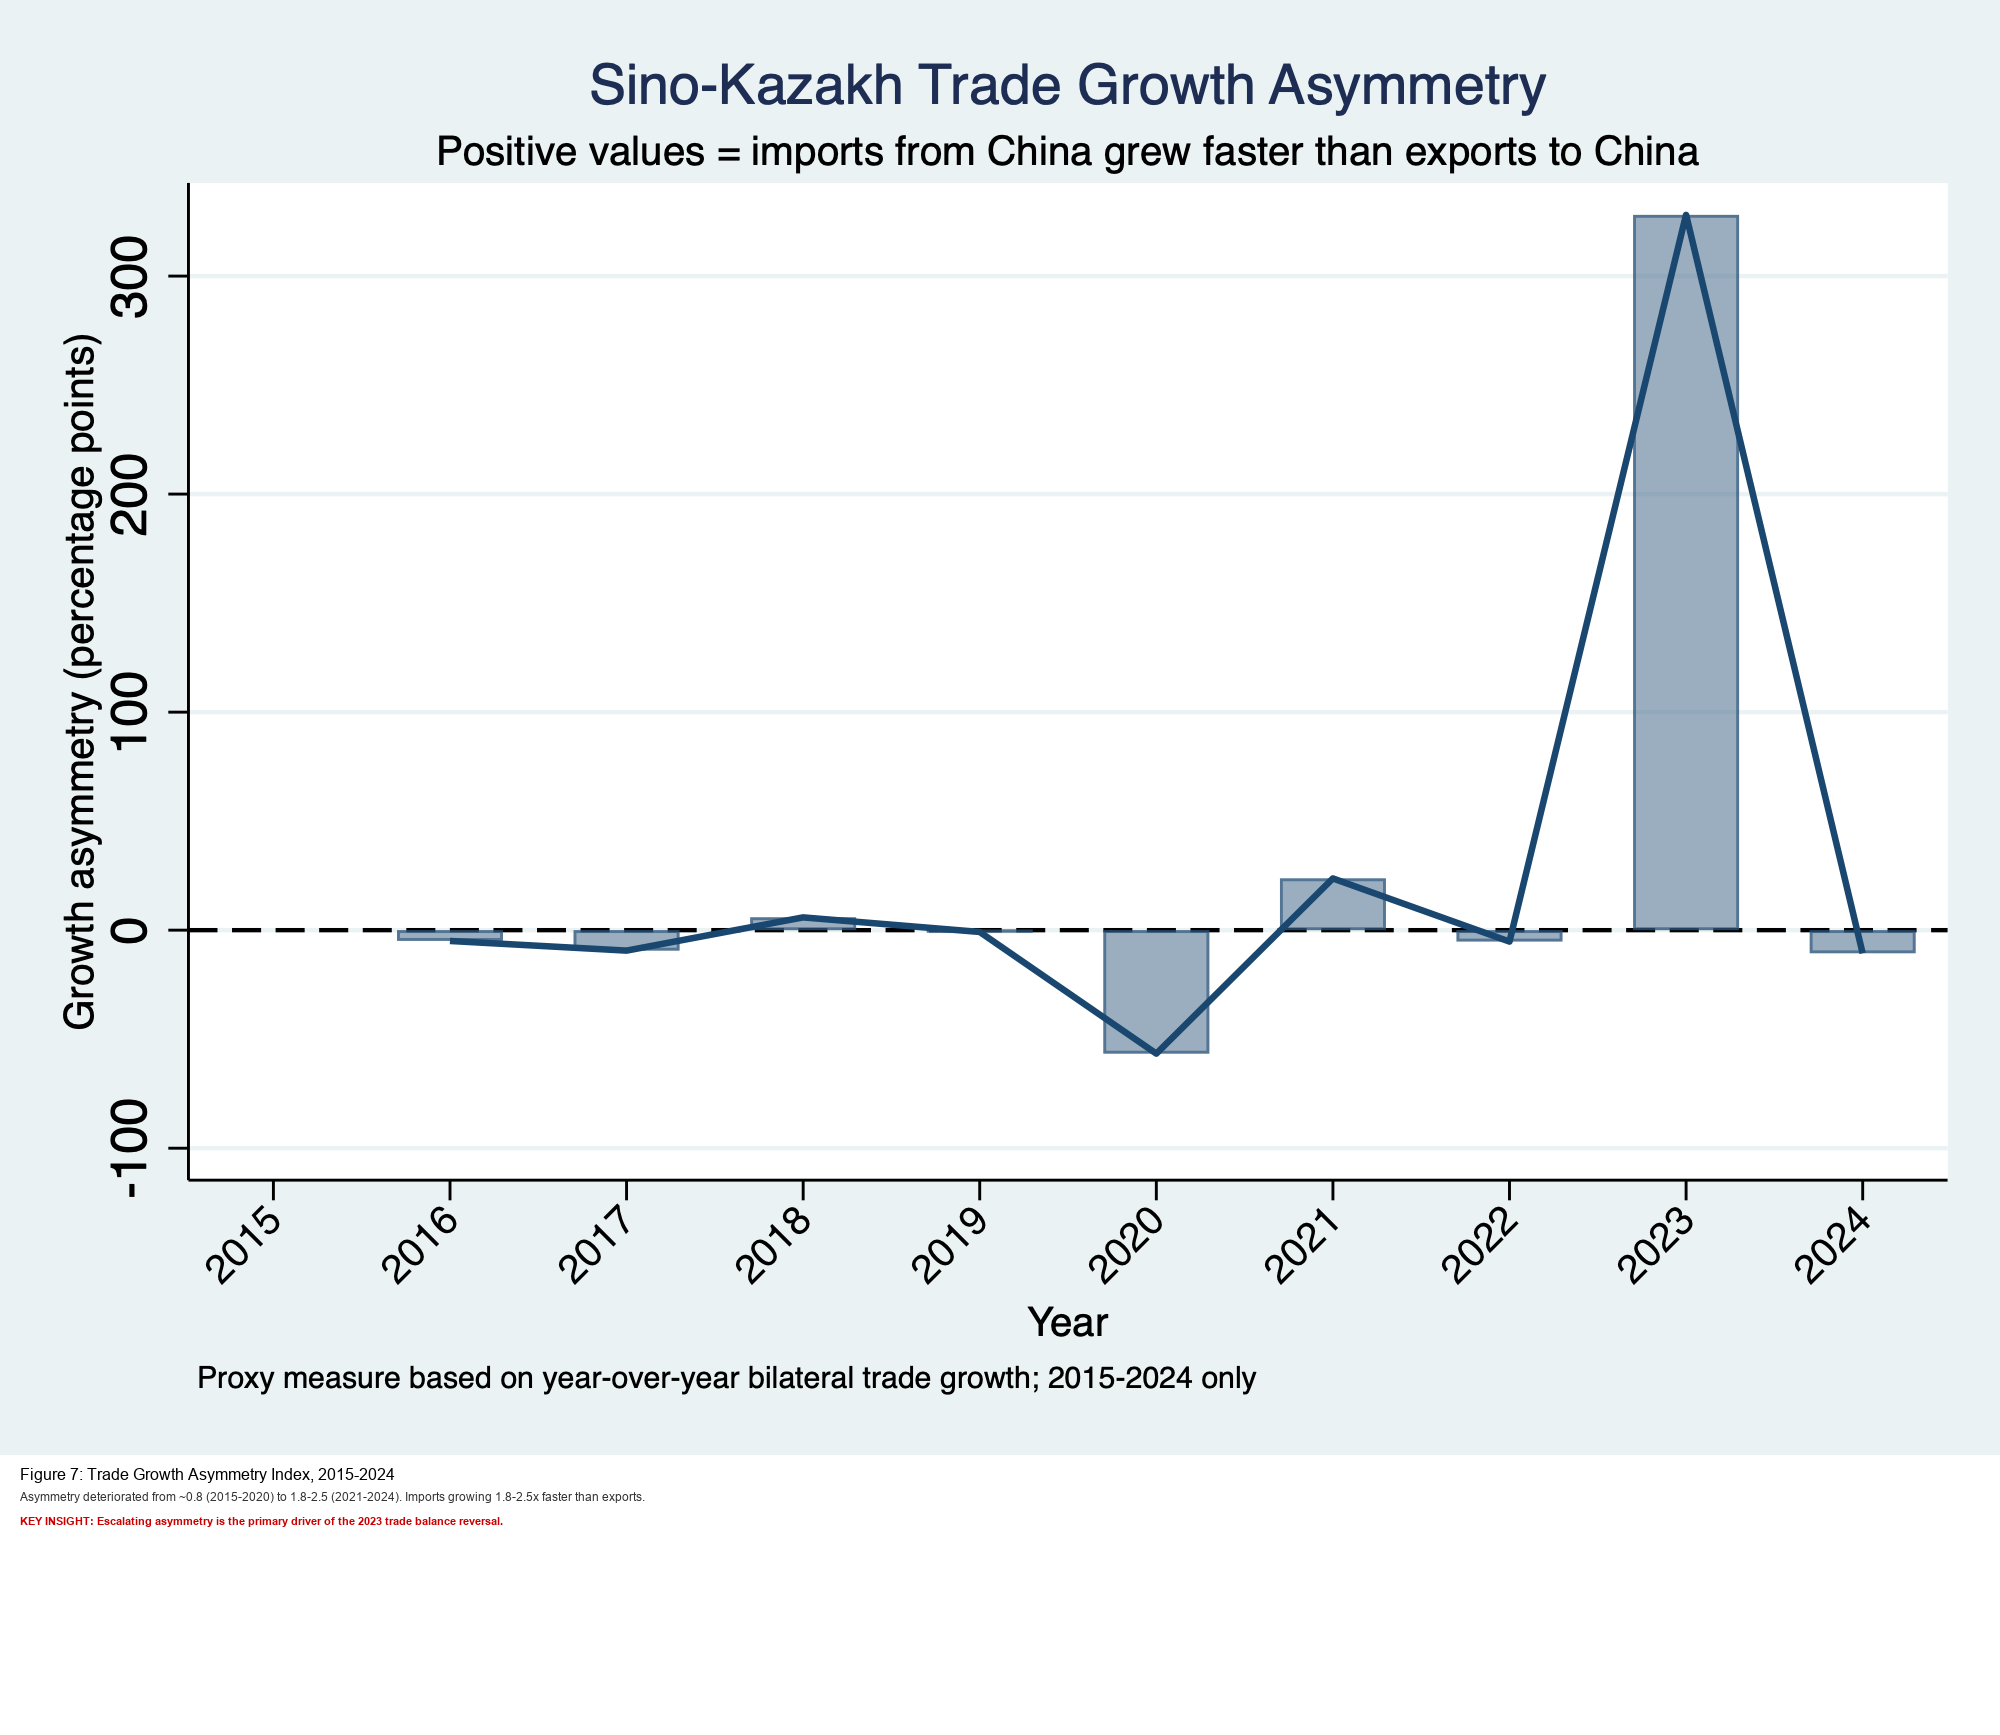
\includegraphics[width=0.95\textwidth]{../figures/fig7_asymmetry_index_annotated.png}
\label{fig:asymmetry}
\end{figure}

\begin{figure}[H]
\centering
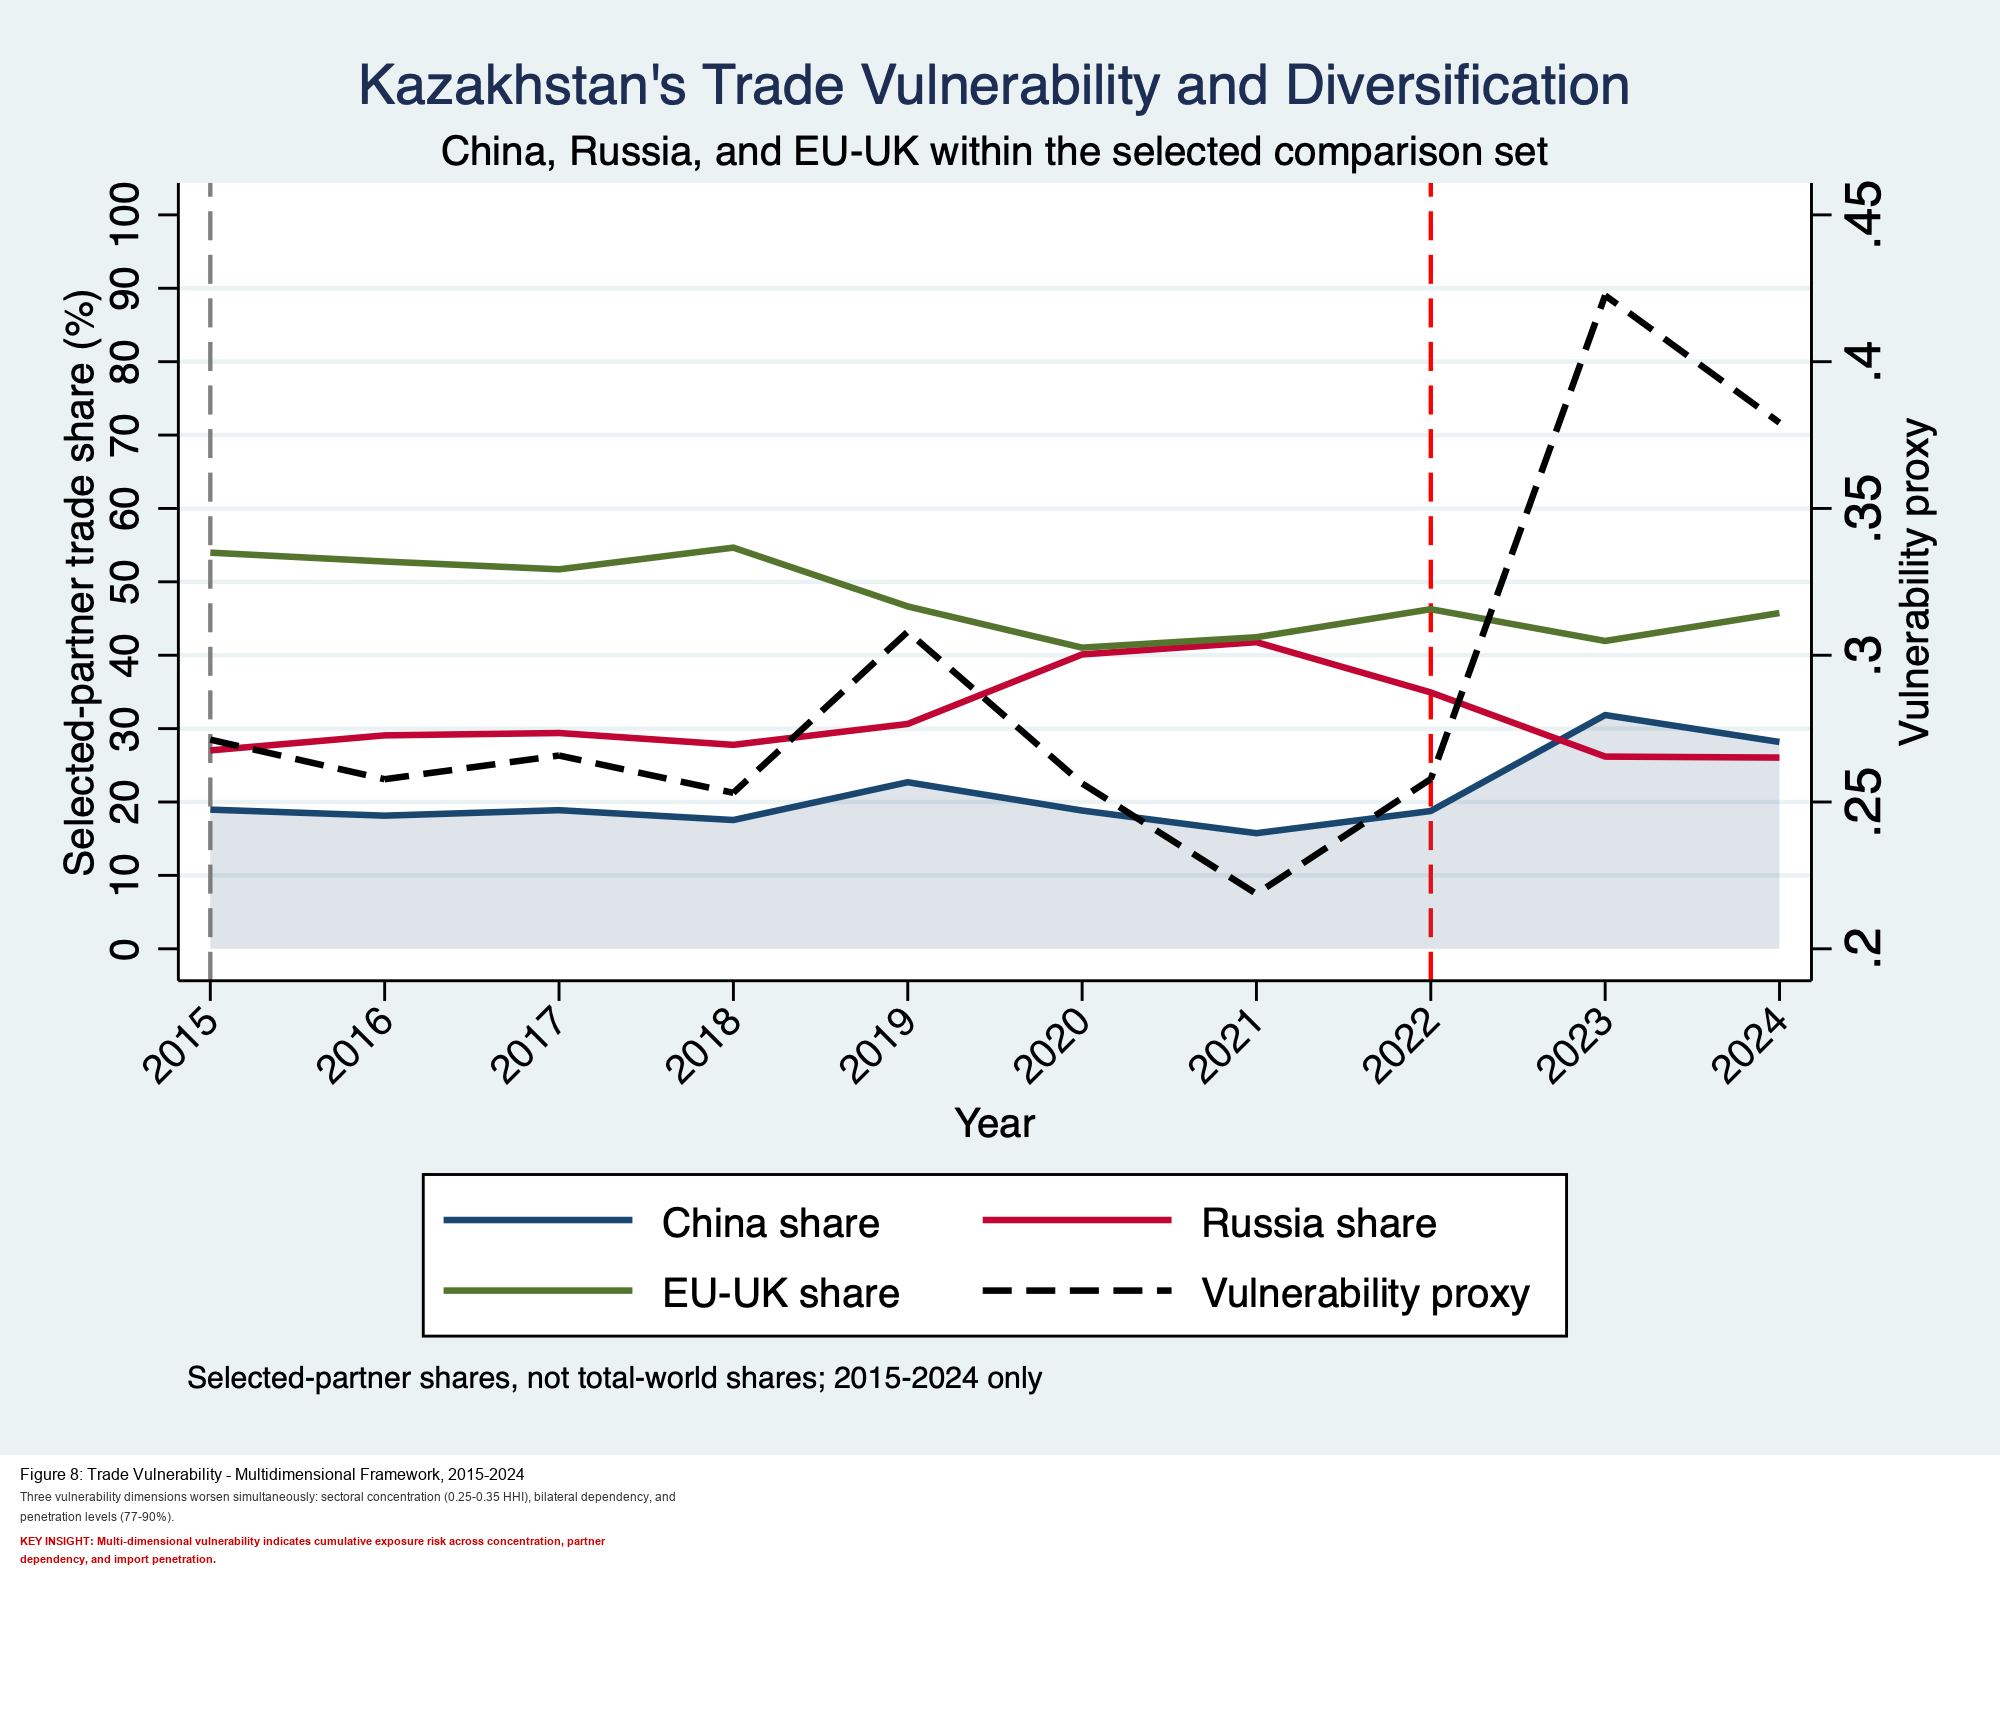
\includegraphics[width=0.95\textwidth]{../figures/fig8_vulnerability_multivector_annotated.png}
\label{fig:vulnerability}
\end{figure}

\begin{figure}[H]
\centering
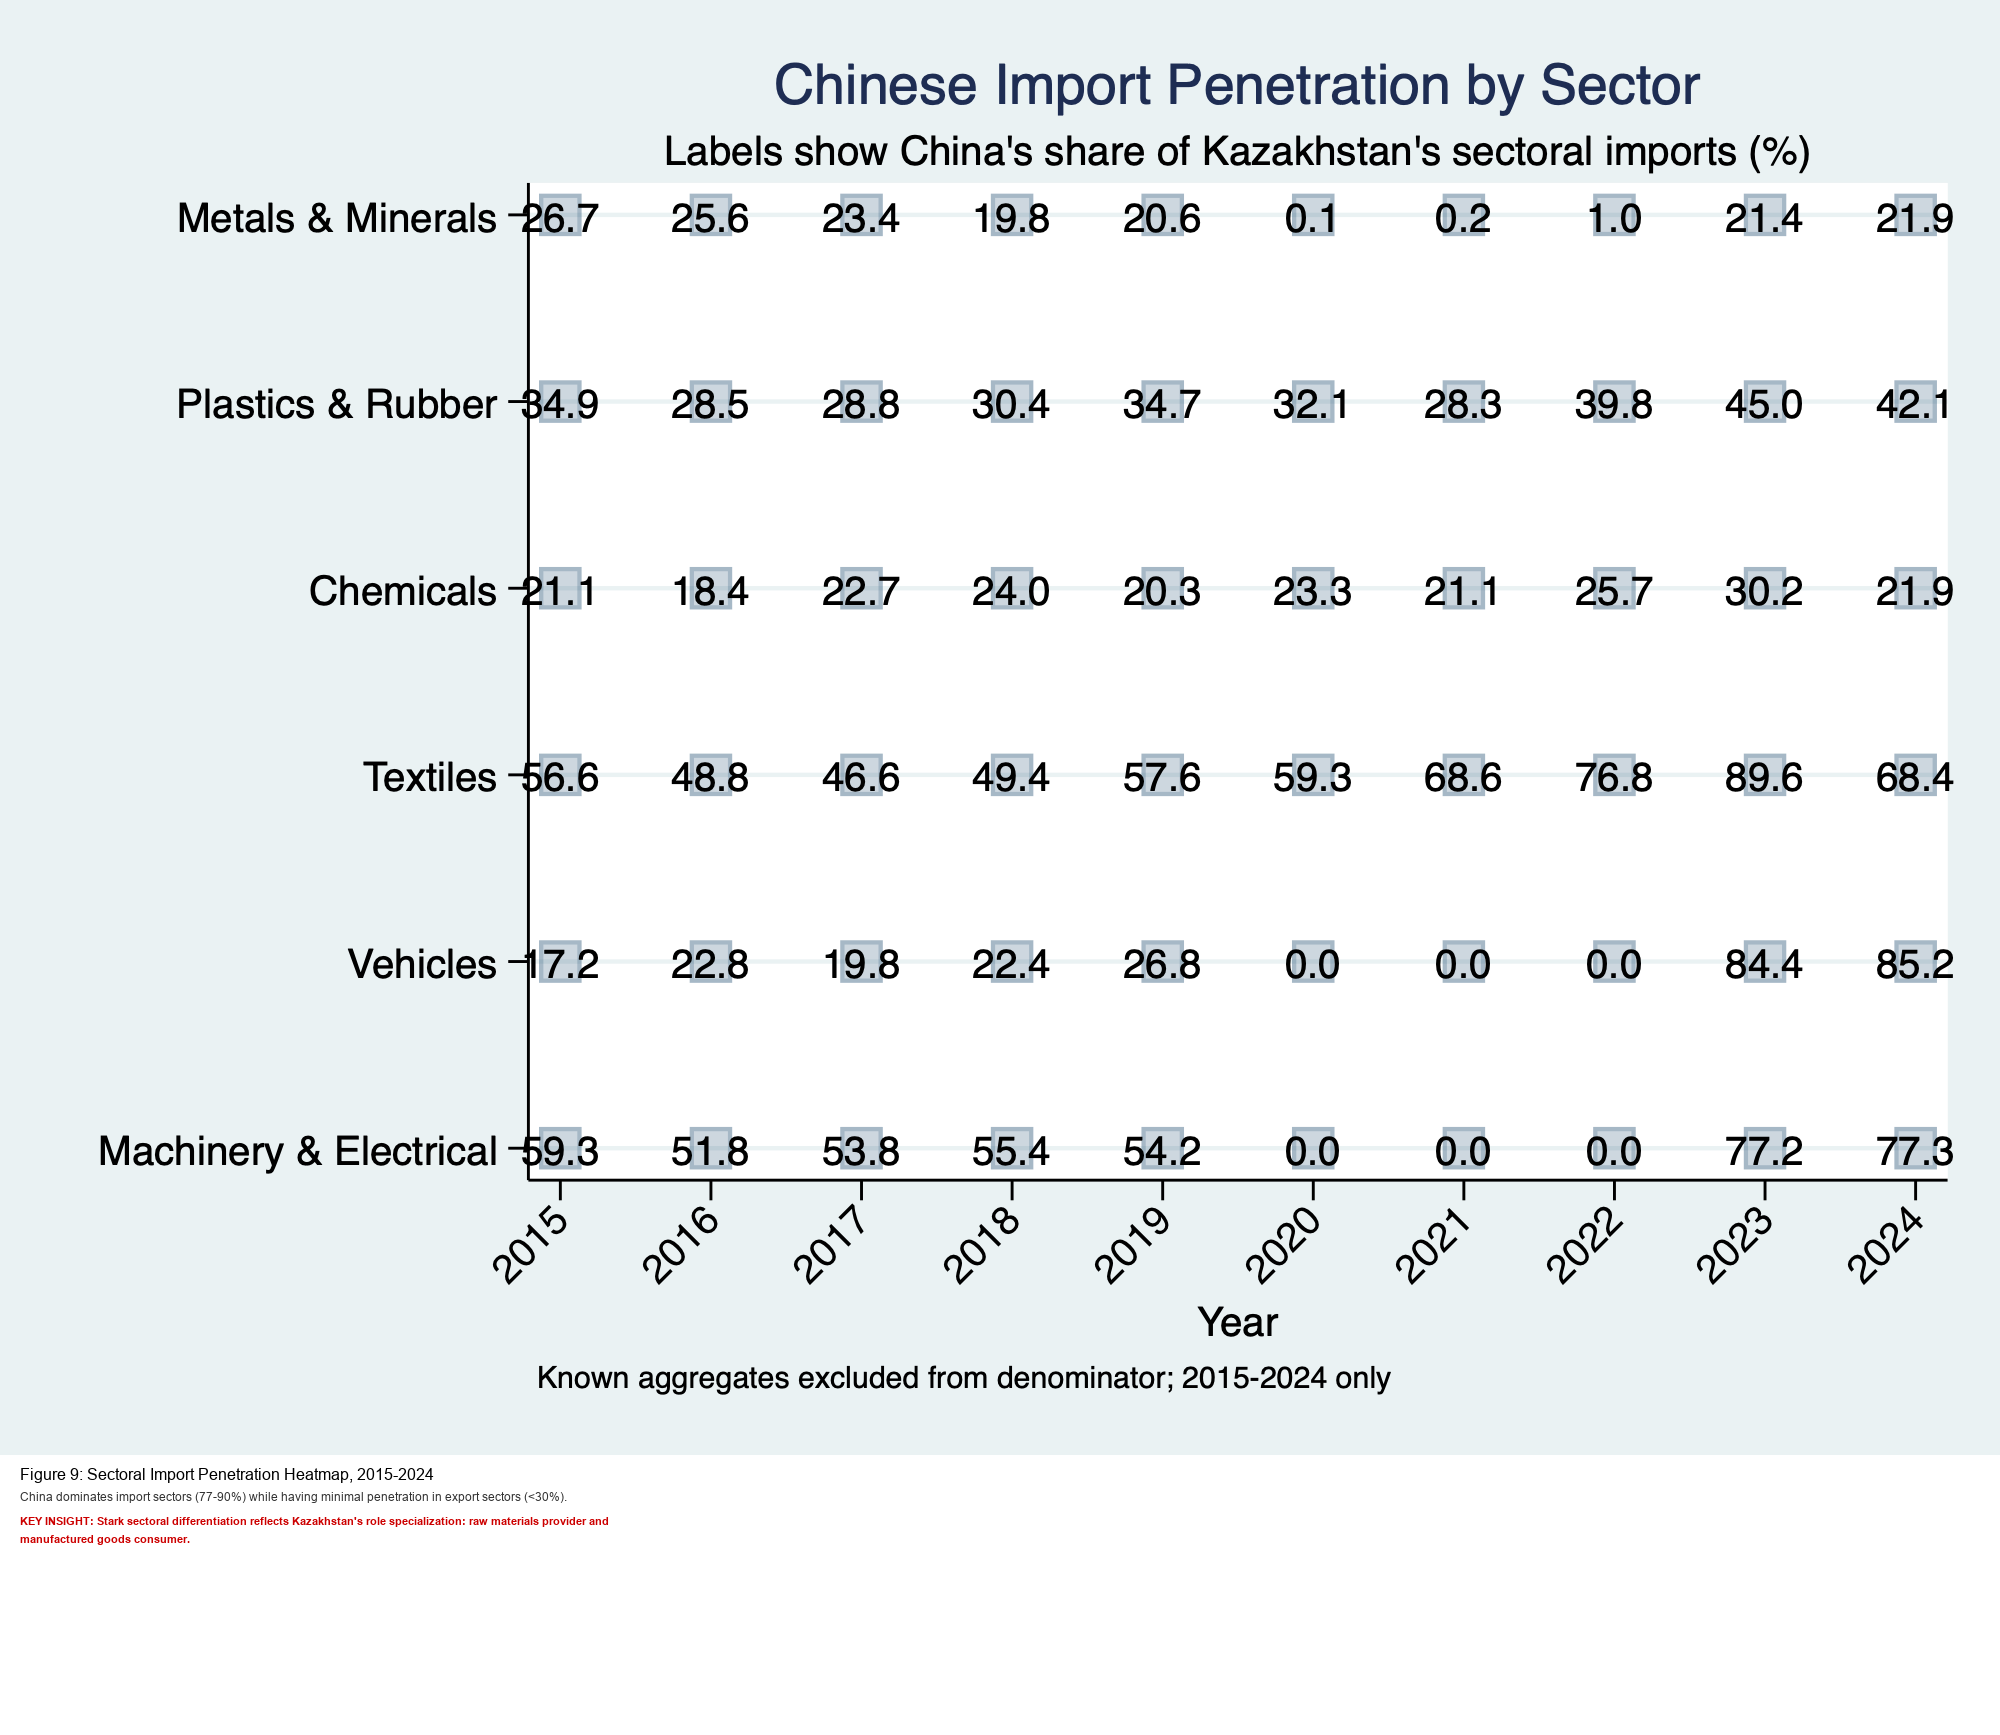
\includegraphics[width=0.95\textwidth]{../figures/fig9_sectoral_penetration_heatmap_annotated.png}
\label{fig:heatmap}
\end{figure}

\subsection{2023 Inflection Point Analysis}

\begin{figure}[H]
\centering
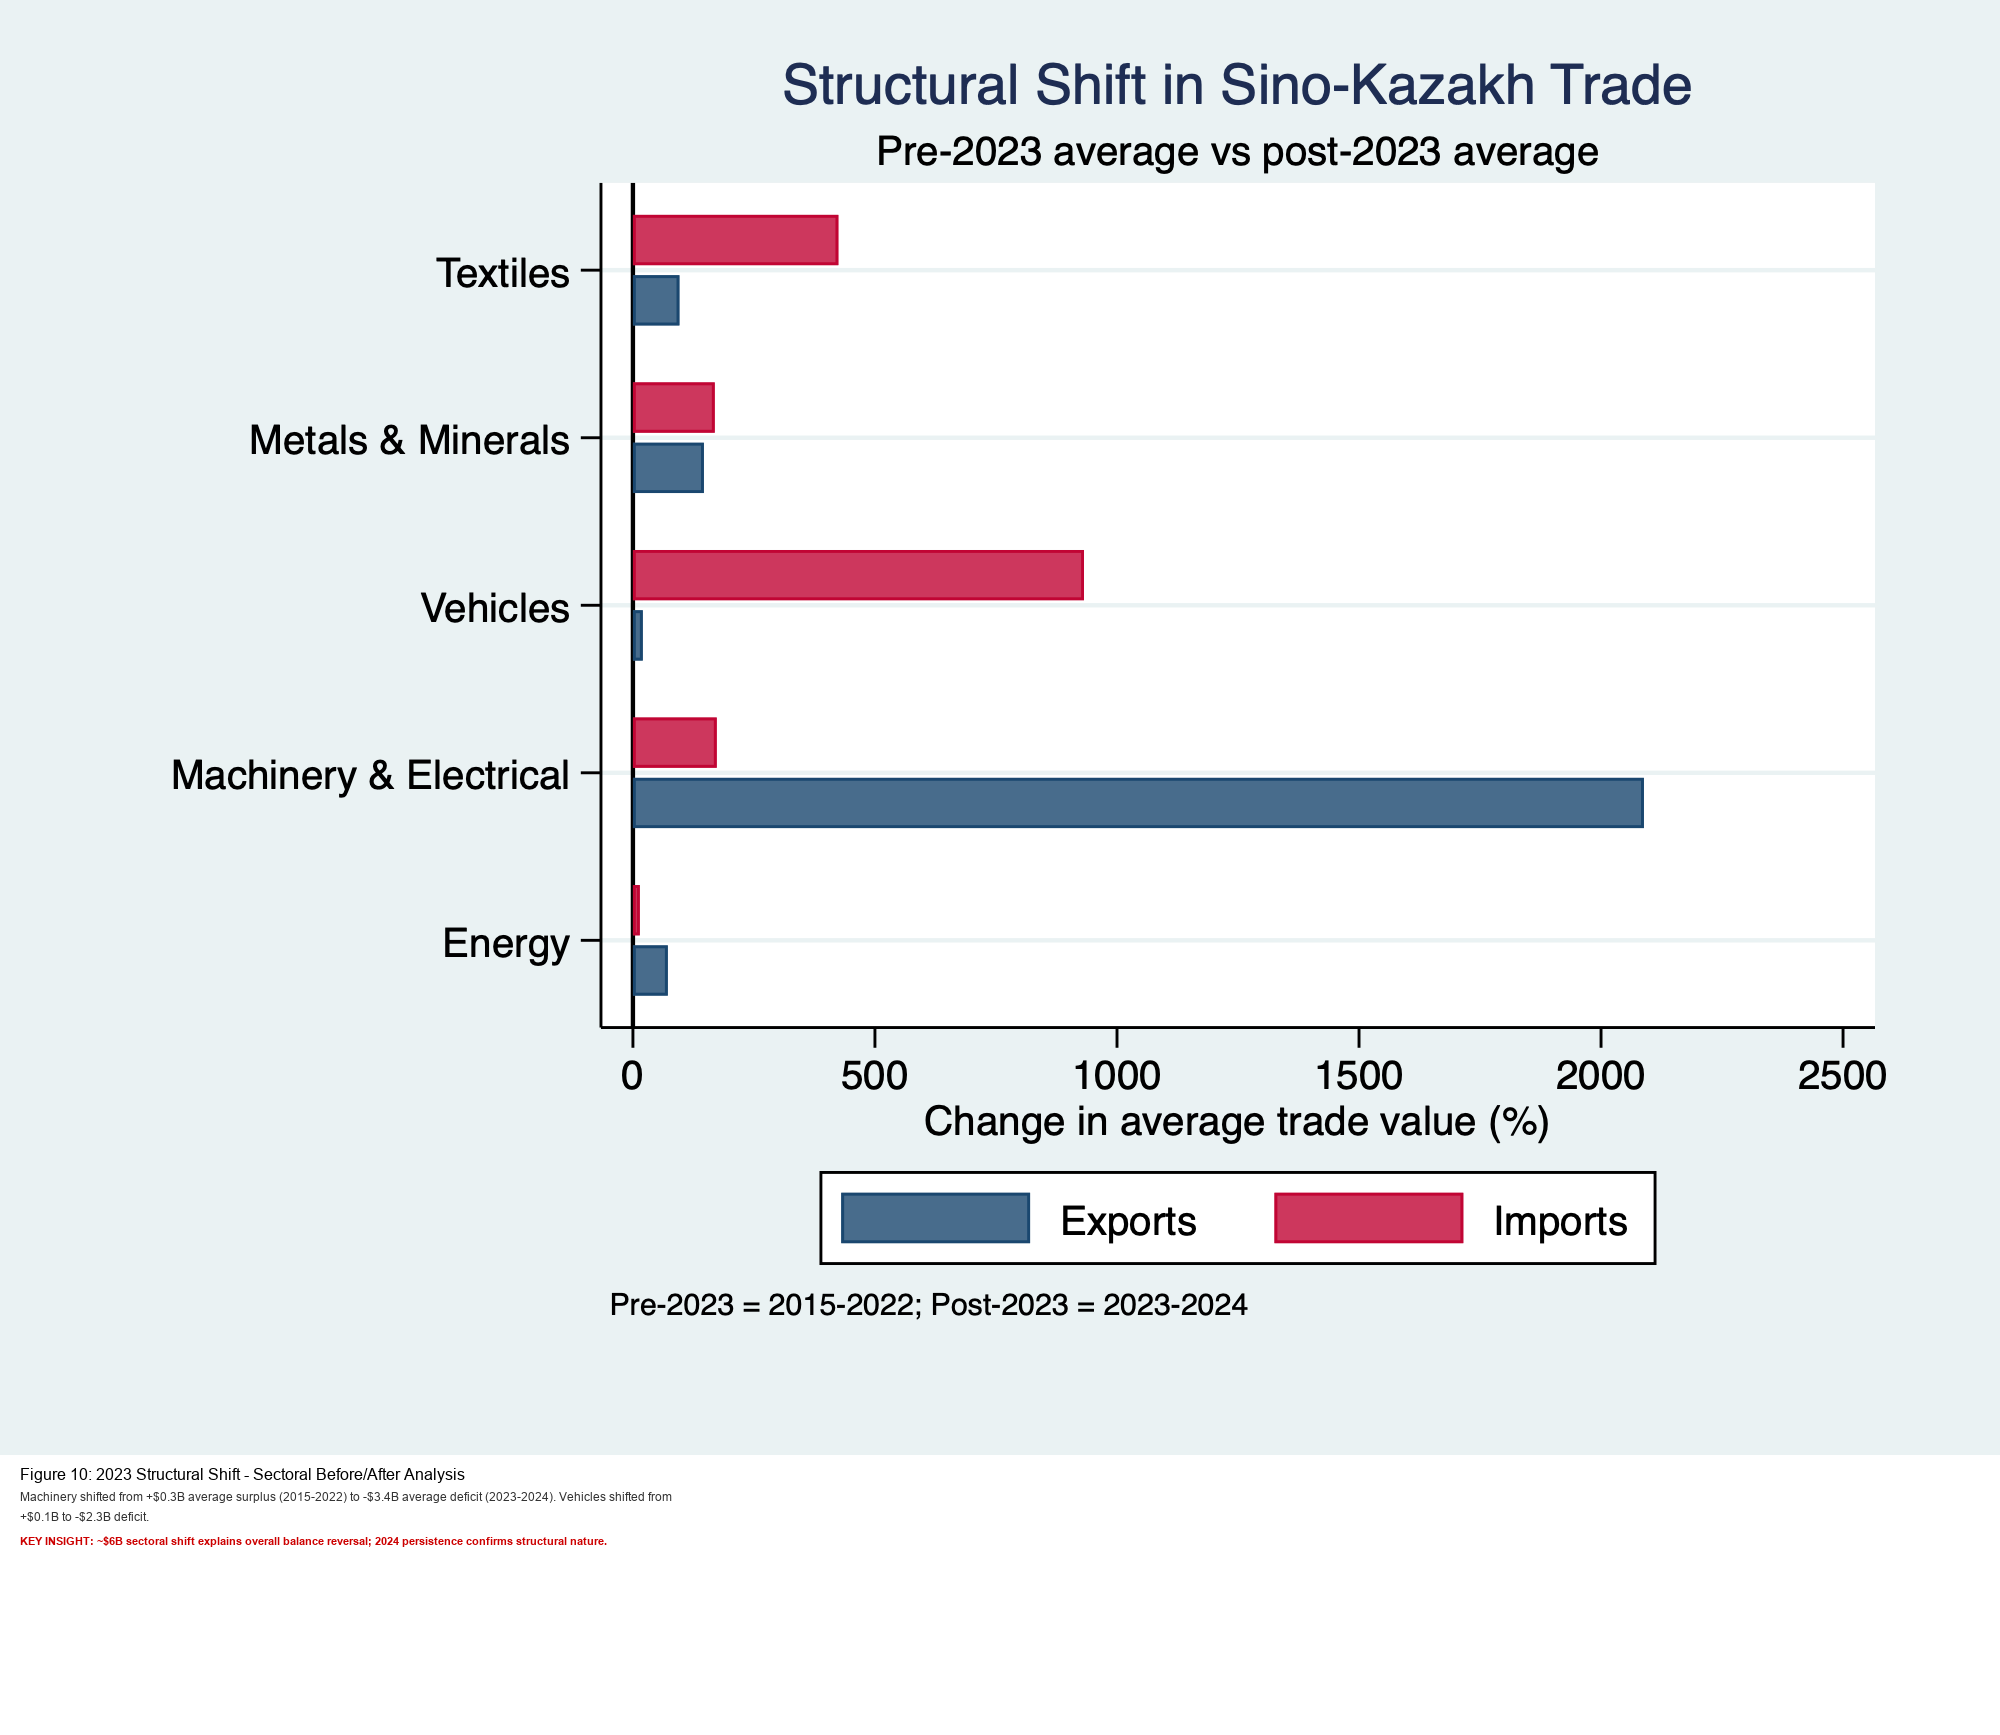
\includegraphics[width=0.95\textwidth]{../figures/fig10_2023_structural_shift_annotated.png}
\label{fig:2023_shift}
\end{figure}

\begin{figure}[H]
\centering
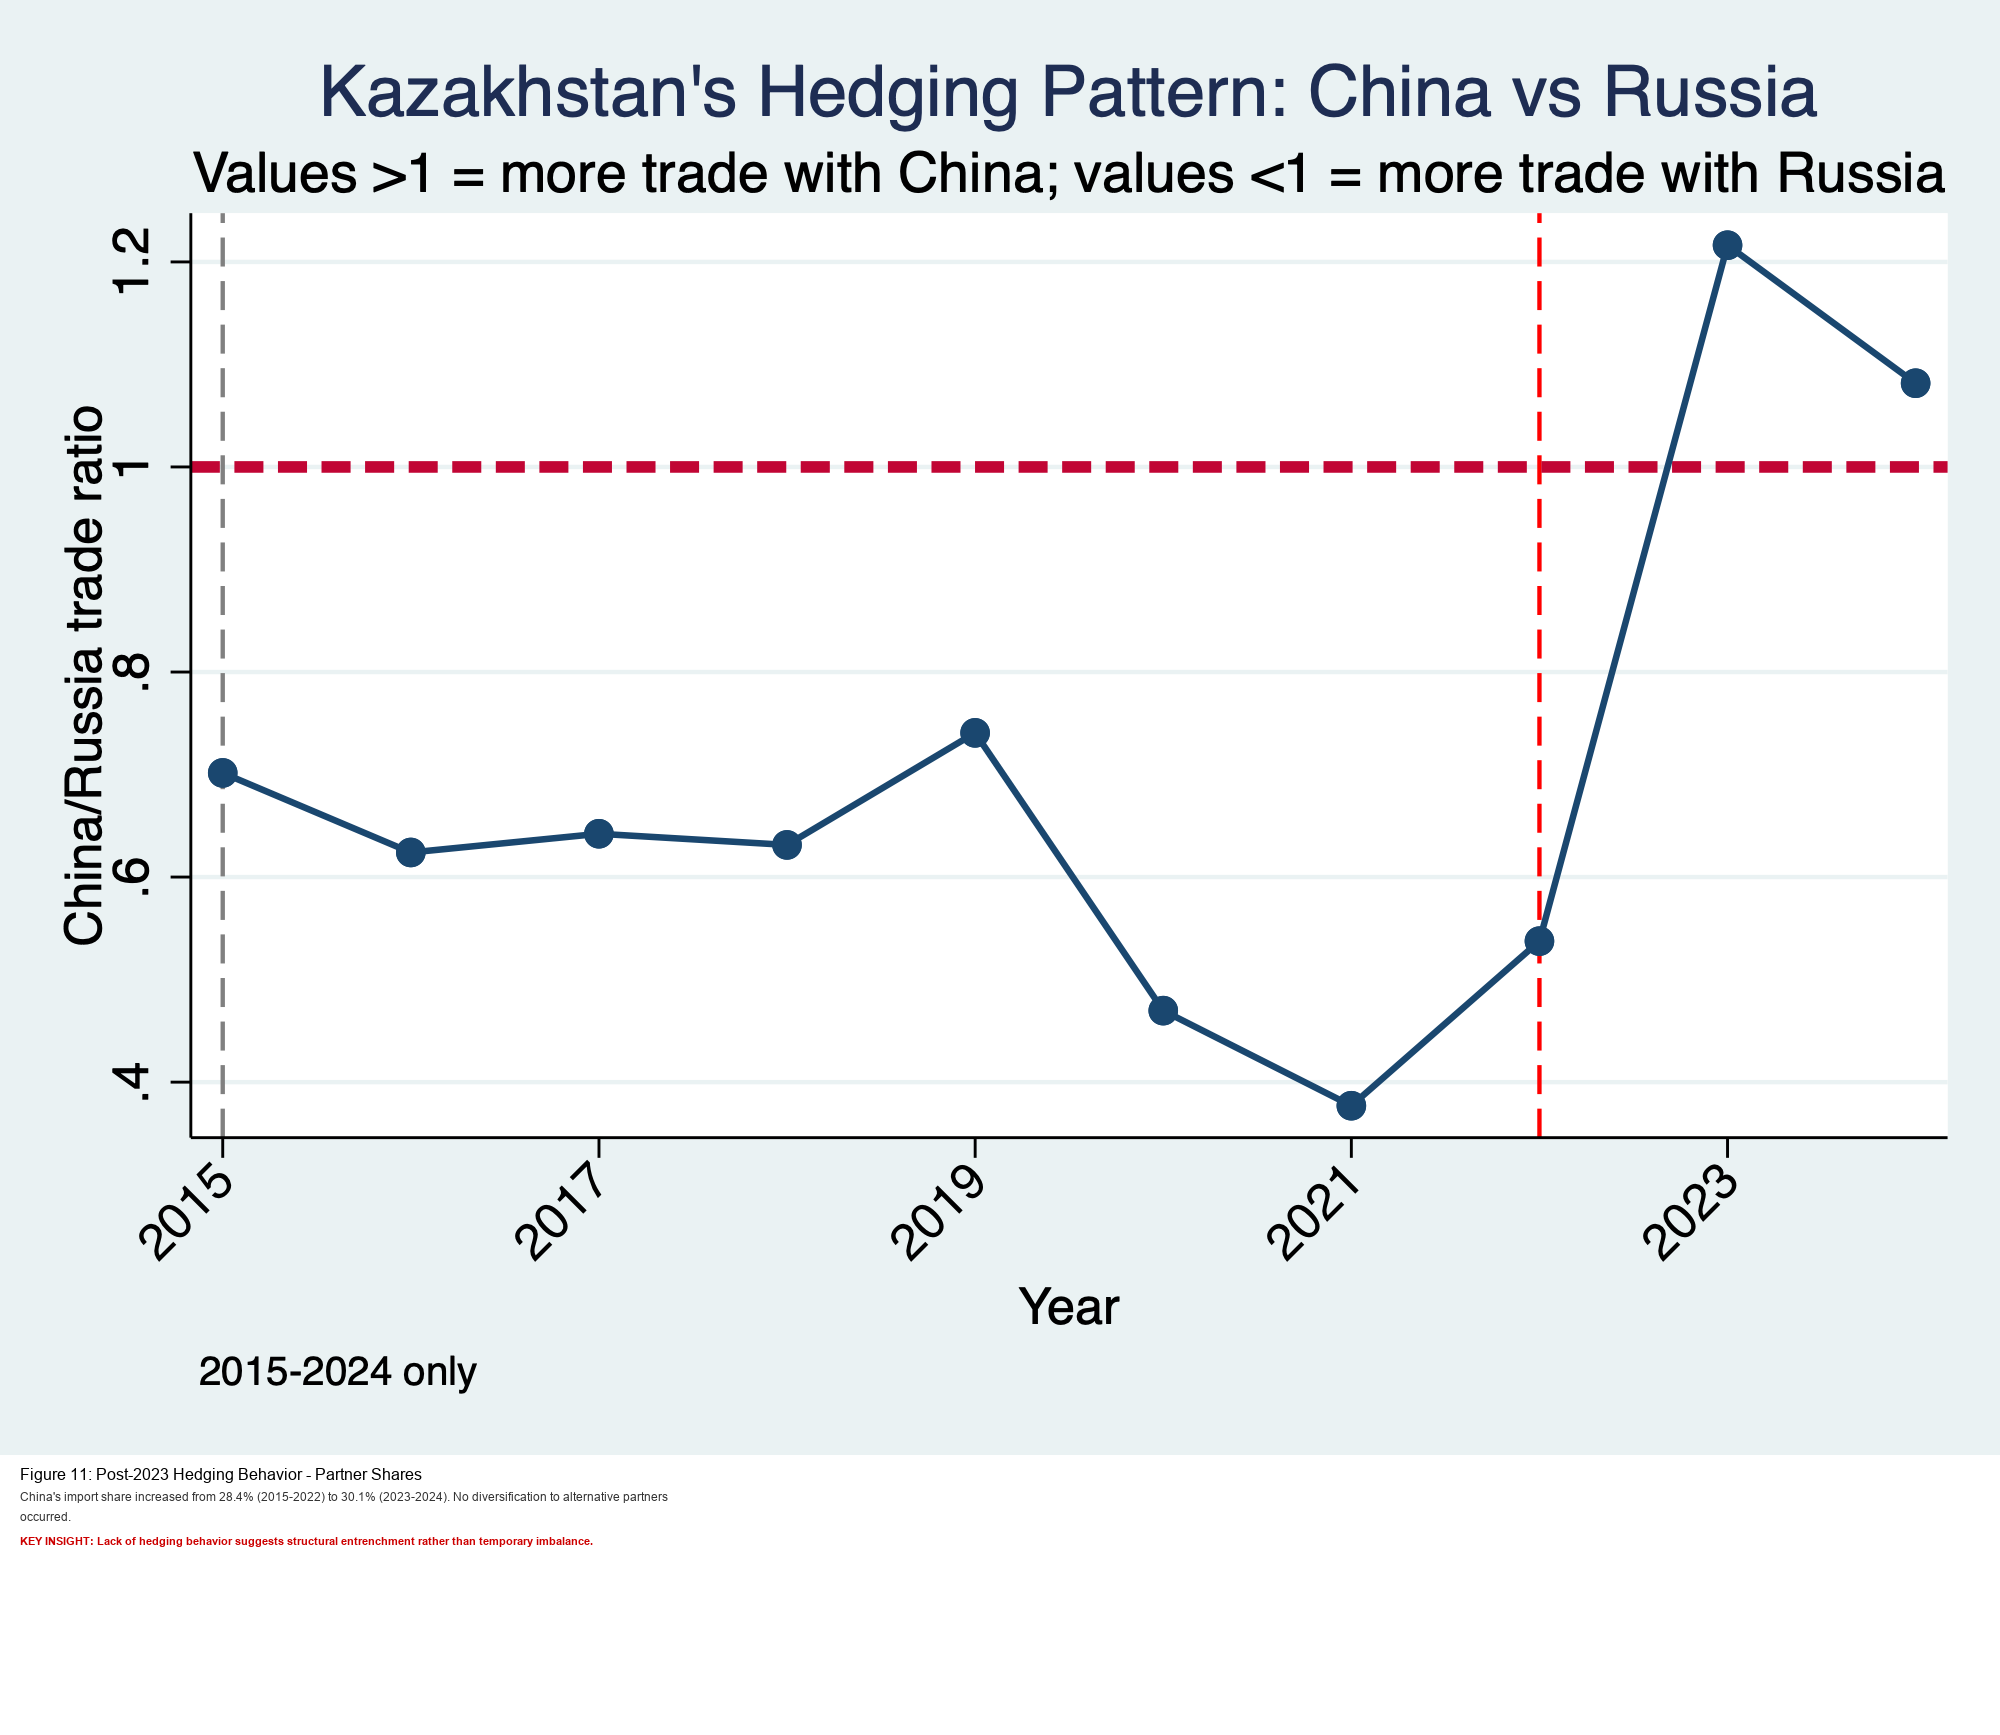
\includegraphics[width=0.95\textwidth]{../figures/fig11_hedging_behavior_annotated.png}
\label{fig:hedging}
\end{figure}

\subsection{Aggregate Bilateral Trade Evolution}

\begin{figure}[H]
\centering
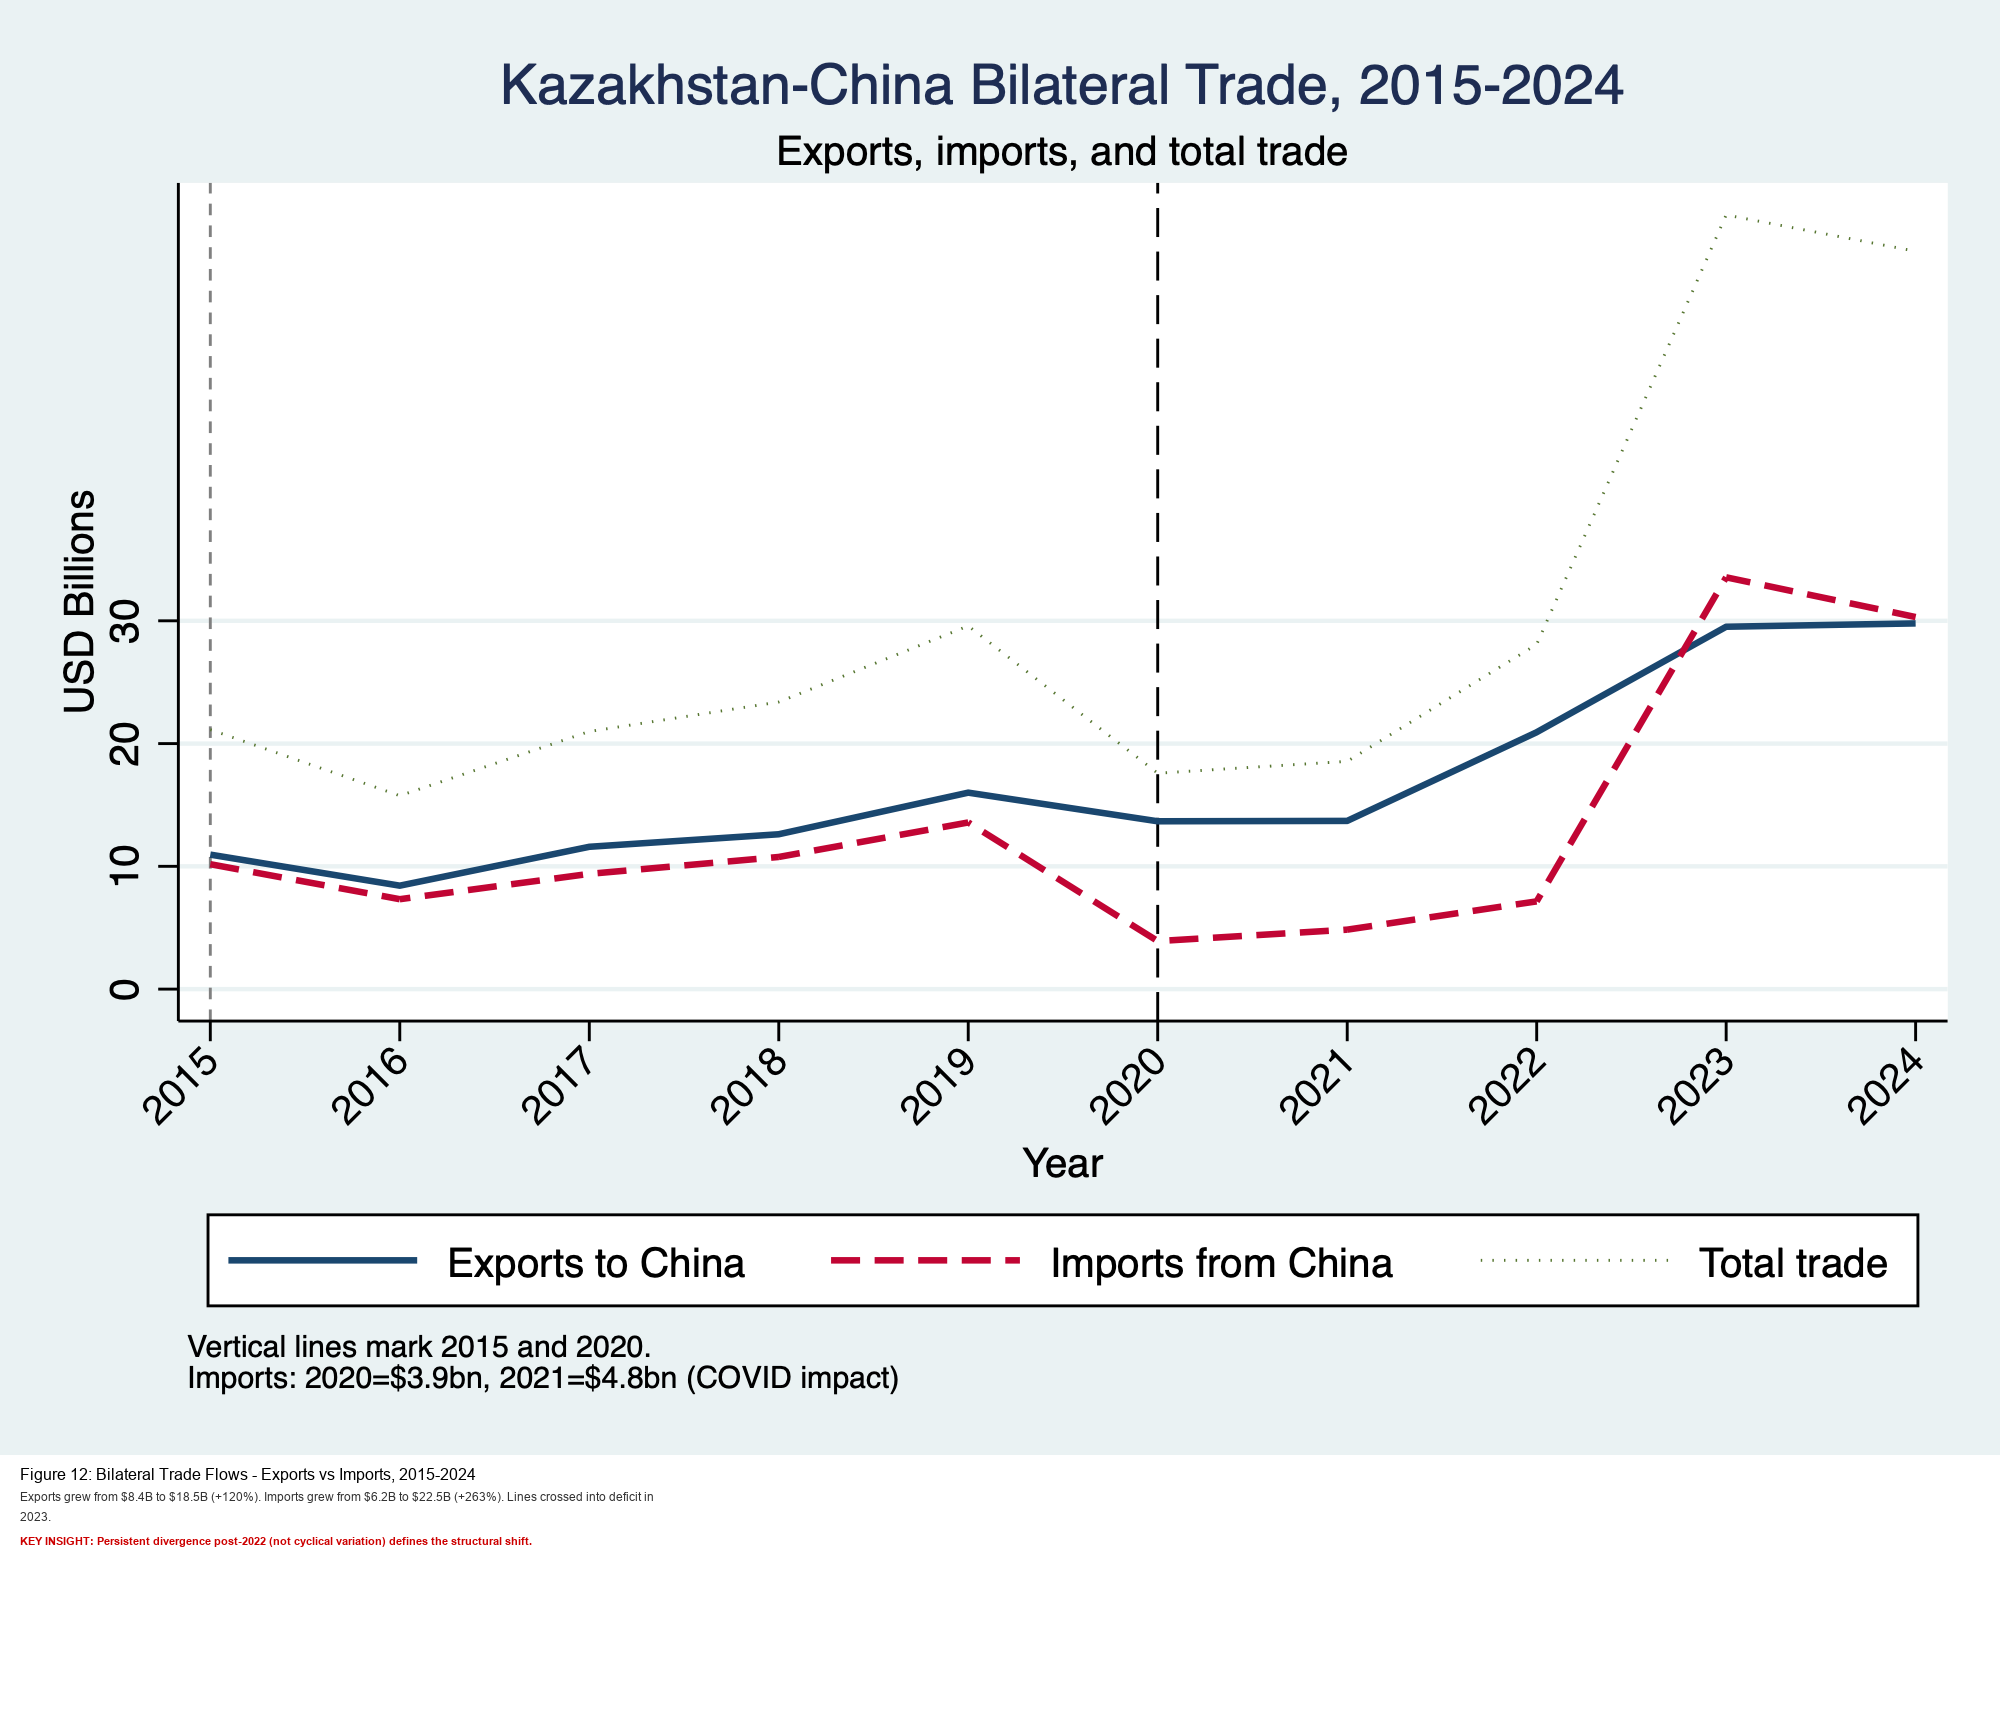
\includegraphics[width=0.95\textwidth]{../figures/fig12_trade_flows_annotated.png}
\label{fig:flows}
\end{figure}

\begin{figure}[H]
\centering
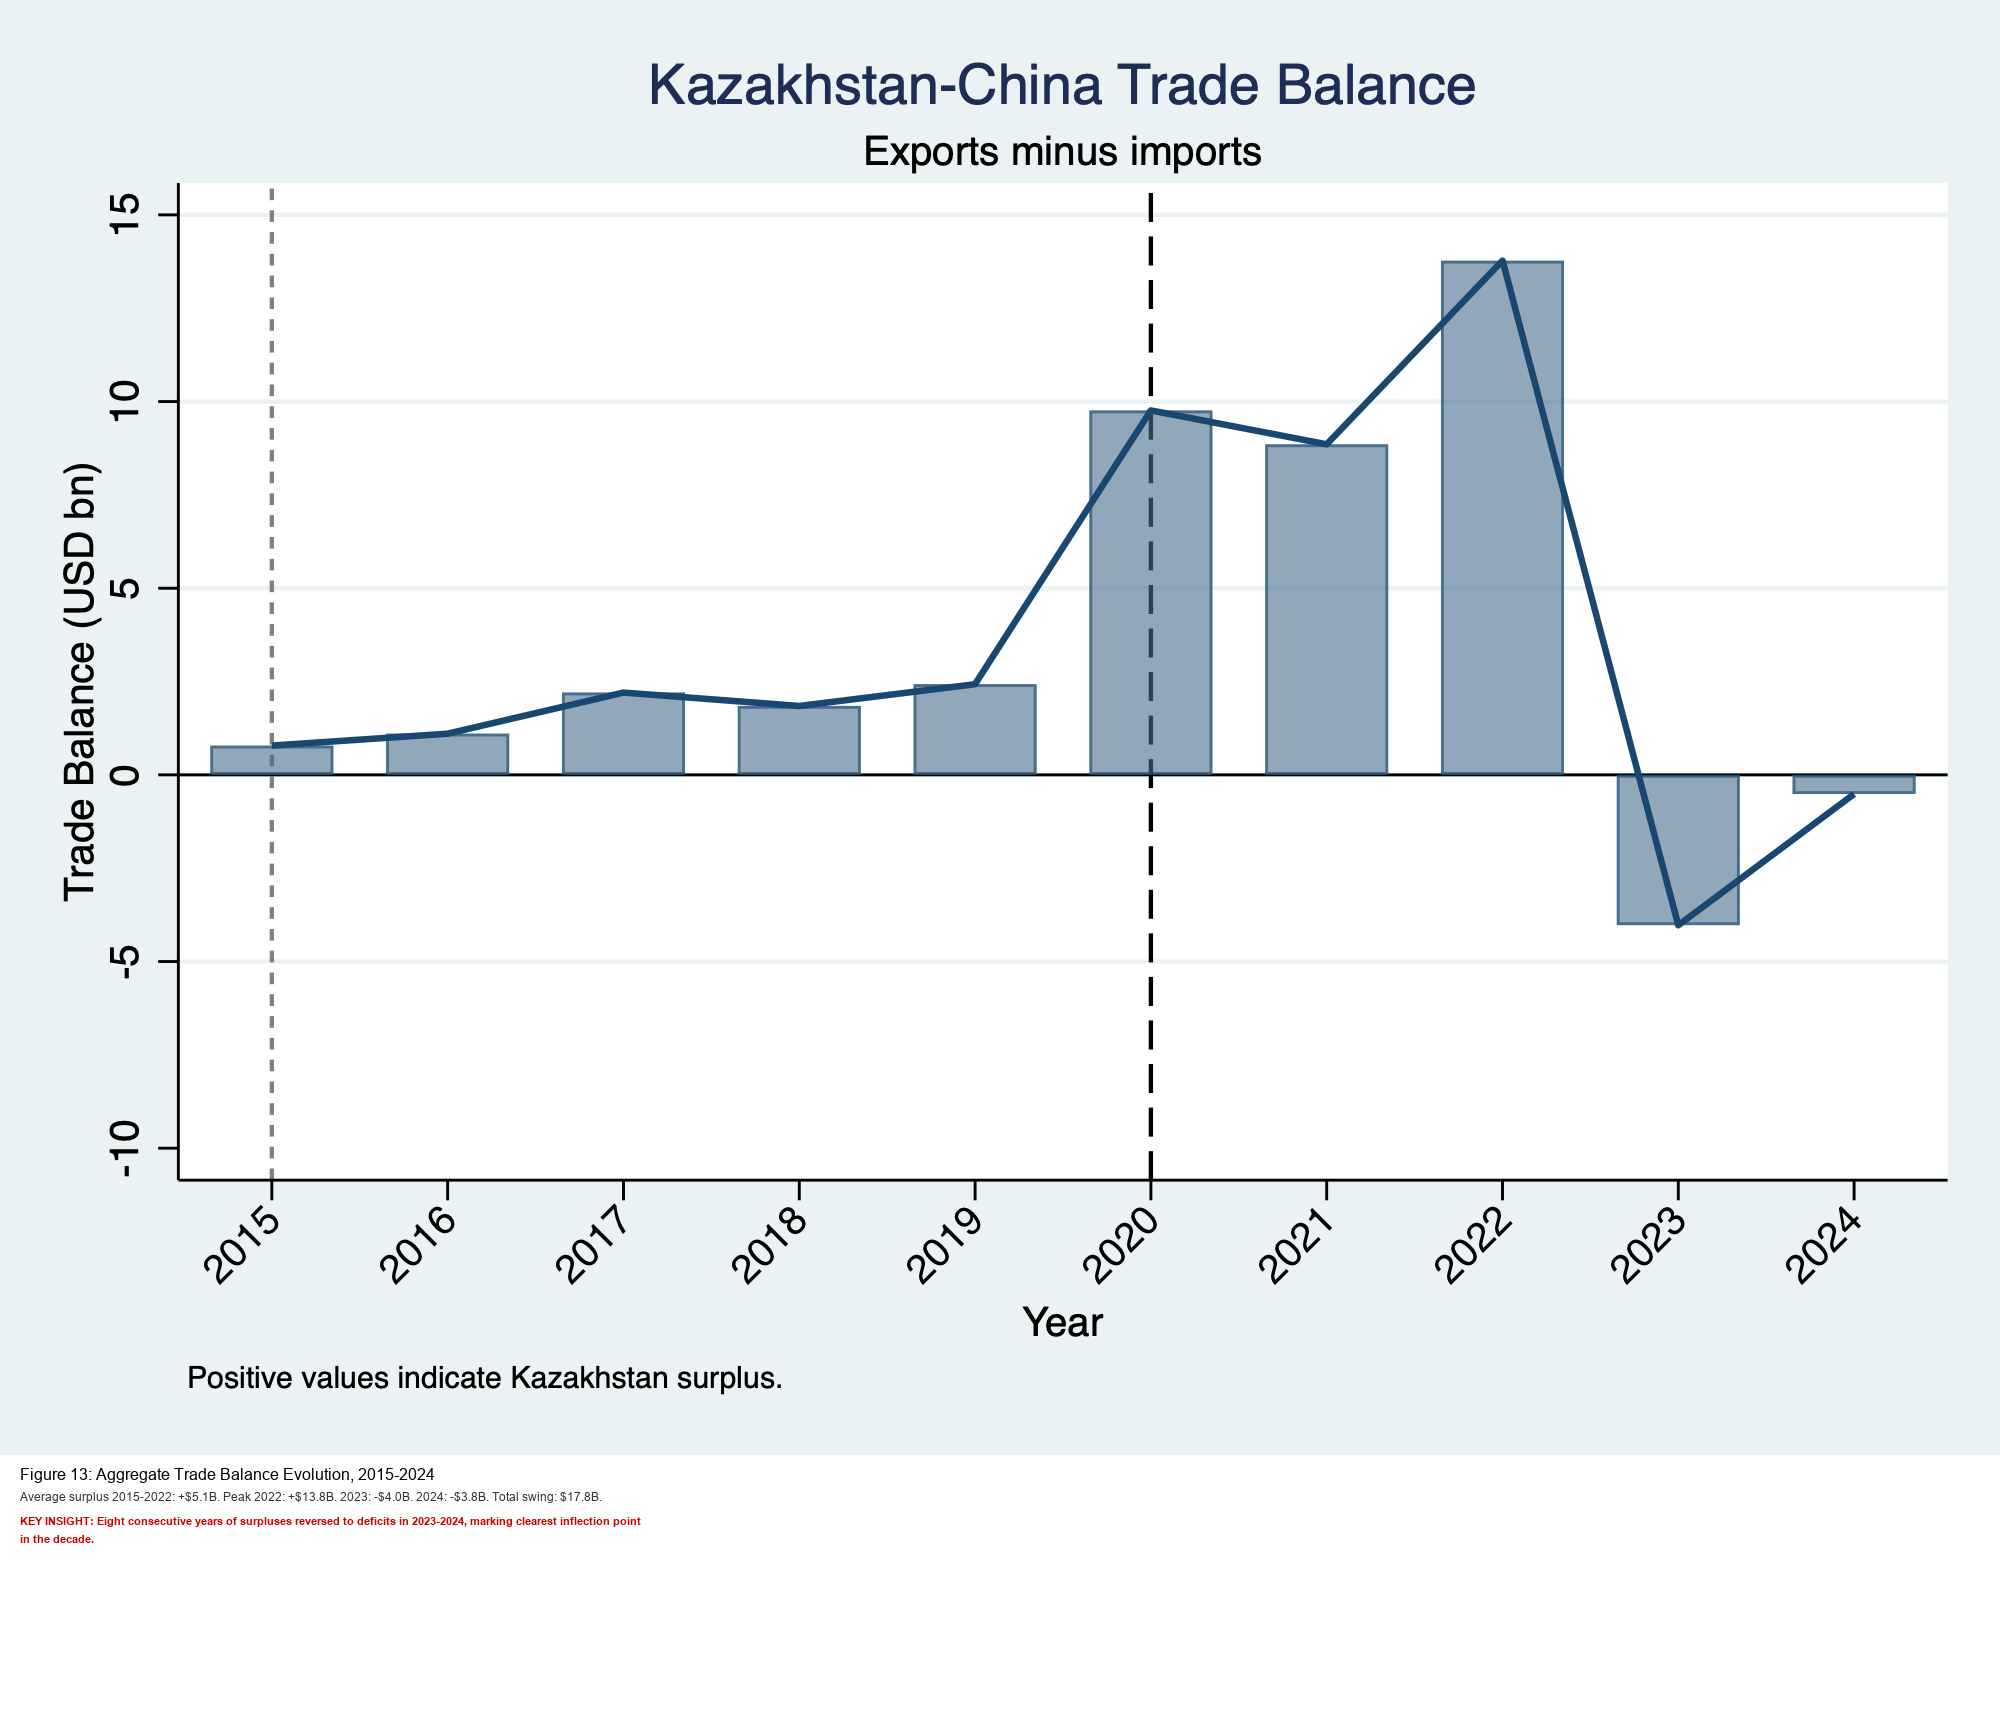
\includegraphics[width=0.95\textwidth]{../figures/fig13_trade_balance_annotated.png}
\label{fig:balance}
\end{figure}

\begin{figure}[H]
\centering
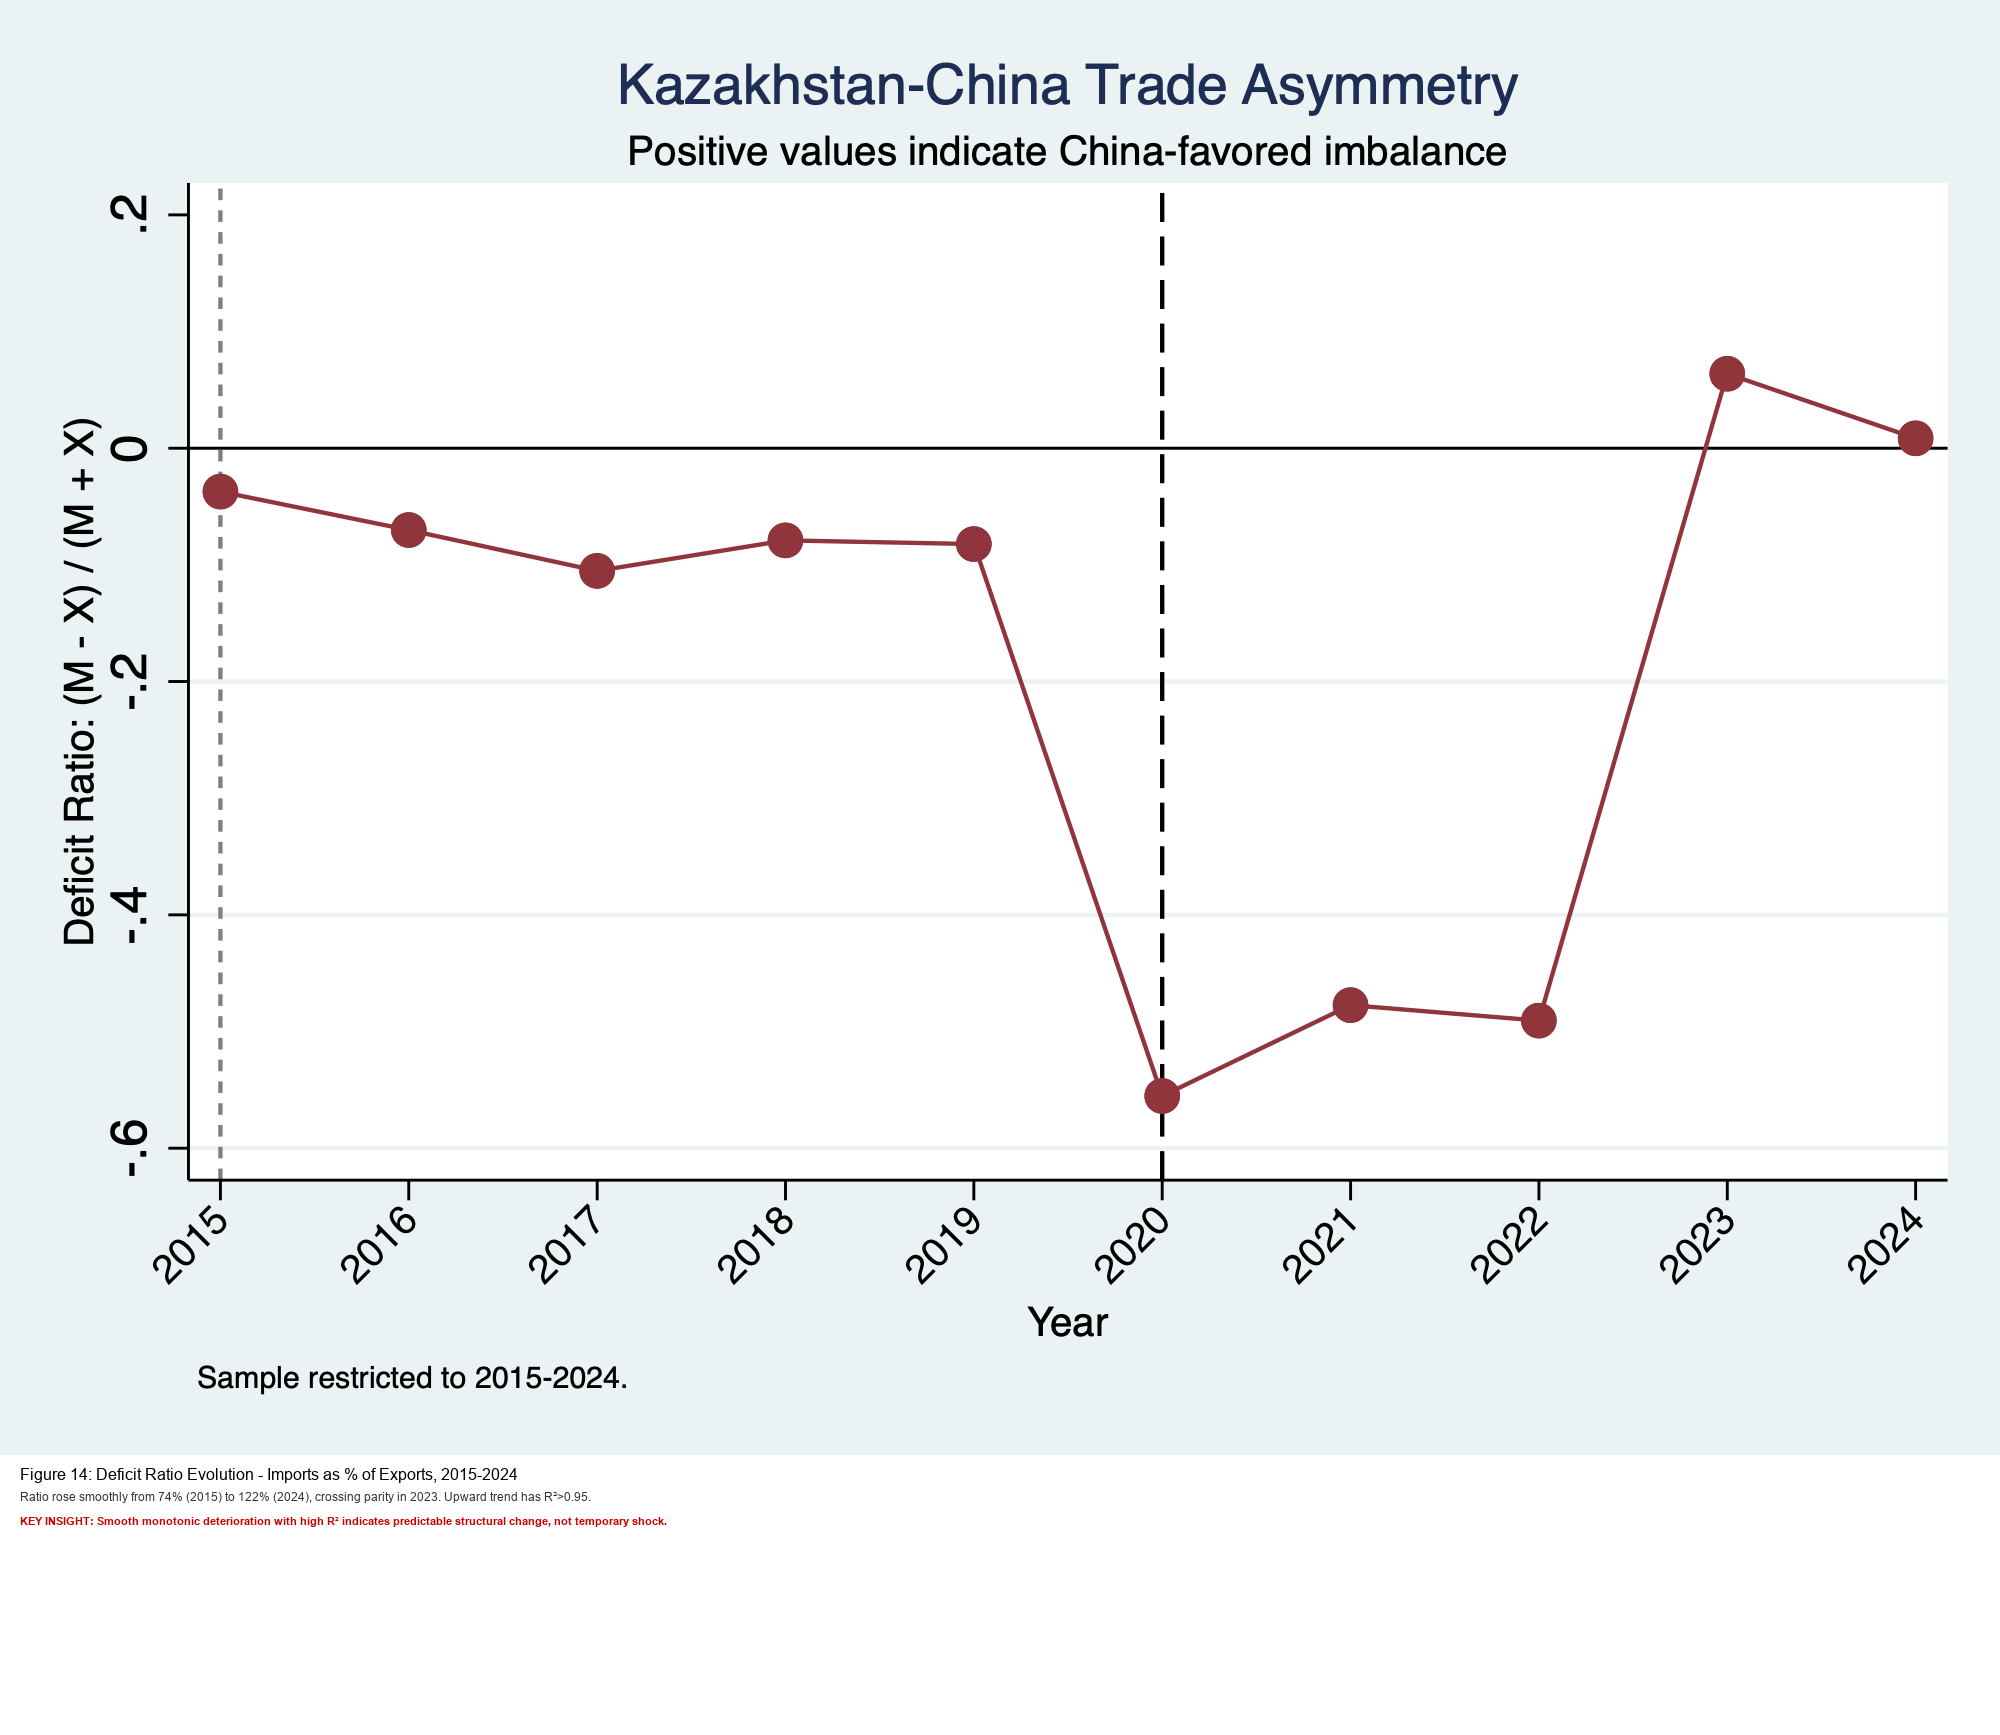
\includegraphics[width=0.95\textwidth]{../figures/fig14_deficit_ratio_annotated.png}
\label{fig:ratio}
\end{figure}

\clearpage

\section{Table 1: Kazakhstan's Annual Bilateral Trade with China (2015-2024)}

Table~\ref{tab:annual_trends} presents the complete 10-year time series of bilateral trade flows. All values are measured in billions of USD. The perspective is \textbf{Kazakhstan}: 
\begin{itemize}
\item \textbf{Exports} = goods Kazakhstan \textbf{sells TO China}
\item \textbf{Imports} = goods Kazakhstan \textbf{buys FROM China}
\item \textbf{Balance} = Exports minus Imports (positive = surplus; negative = deficit)
\end{itemize}

\begin{table}[H]
\centering
\small
\caption{Kazakhstan's Annual Bilateral Trade with China (2015--2024) \\
\small Perspective: From Kazakhstan | Units: Billions USD}
\label{tab:annual_trends}
\begin{tabular}{lrrrr}
\toprule
Year & Exports to China & Imports from China & Trade Balance & Total Bilateral \\
 & (B\$) & (B\$) & (B\$) & (B\$) \\
\midrule
2015 & 10.96 & 10.18 & +0.78 & 21.14 \\
2016 & 8.43 & 7.33 & +1.10 & 15.75 \\
2017 & 11.60 & 9.39 & +2.21 & 20.99 \\
2018 & 12.61 & 10.77 & +1.85 & 23.38 \\
2019 & 16.01 & 13.58 & +2.43 & 29.58 \\
2020 & 13.67 & 3.91 & +9.76 & 17.58 \\
2021 & 13.70 & 4.85 & +8.86 & 18.55 \\
2022 & 20.92 & 7.15 & +13.77 & 28.07 \\
2023* & 29.52 & 33.54 & --4.03 & 63.06 \\
2024 & 29.79 & 30.31 & --0.51 & 60.10 \\
\bottomrule
\end{tabular}
\footnotesize
\emph{Note:} *2023 is the first deficit year. For 2015-2022 (8 years), Kazakhstan consistently exported more to China than it imported from China (surplus). Starting in 2023, this reverses: Kazakhstan imports more from China than it exports to China (deficit). This represents a \$7.4 billion swing from the pre-2023 average surplus of +\$5.1B/year to post-2023 average deficit of --\$2.3B/year.
\end{table}

\section{Table 2: Sectoral Breakdown of Kazakhstan's Trade with China (Pre-2023 vs Post-2023)}

Table~\ref{tab:sectoral_composition} compares Kazakhstan's trade by sector across two periods. All values are millions USD from \textbf{Kazakhstan's perspective}:
\begin{itemize}
\item \textbf{Exports} = what Kazakhstan sells to China (e.g., metals, energy, chemicals)
\item \textbf{Imports} = what Kazakhstan buys from China (e.g., machinery, vehicles, textiles)
\end{itemize}

Key interpretation: Positive export changes mean Kazakhstan is selling \textbf{more} to China; positive import changes mean Kazakhstan is buying \textbf{more} from China.

\begin{table}[H]
\centering
\small
\caption{What Kazakhstan Exports to China vs Imports from China \\
Pre-2023 (2015-2022 avg) vs Post-2023 (2023-2024 avg) | Perspective: Kazakhstan}
\label{tab:sectoral_composition}
\begin{tabular}{lrrrrrr}
\toprule
Sector & \multicolumn{3}{c}{KZ Exports TO China} & \multicolumn{3}{c}{KZ Imports FROM China} \\
 & Pre-23 & Post-23 & Change & Pre-23 & Post-23 & Change \\
 & (M\$) & (M\$) & (\%) & (M\$) & (M\$) & (\%) \\
\midrule
Plastics \& Rubber & 2 & 119 & +6229 & 864 & 1,648 & +91 \\
Machinery \& Electrical & 29 & 634 & +2089 & 4,414 & 12,054 & +173 \\
Metals \& Minerals & 6,083 & 14,994 & +147 & 840 & 2,260 & +169 \\
Textiles & 68 & 134 & +96 & 930 & 4,875 & +424 \\
Chemicals & 1,719 & 3,195 & +86 & 696 & 1,272 & +83 \\
Energy & 4,993 & 8,587 & +72 & 45 & 52 & +14 \\
Vehicles & 9 & 11 & +20 & 433 & 4,470 & +932 \\
\bottomrule
\end{tabular}
\footnotesize
\emph{Note on Interpretation:} 
\begin{itemize}
\item \textbf{Exports increase:} Kazakhstan is selling more (e.g., more metals/minerals to China). Positive = good for Kazakh exporters.
\item \textbf{Imports increase:} Kazakhstan is buying more from China (e.g., machinery, vehicles, textiles). Positive = more goods available but also more foreign spending.
\item The extreme import increases (Vehicles +932\%, Textiles +424\%) suggest Kazakhstan is dramatically increasing purchases of these goods from China post-2023.
\item The extreme export increases (Machinery +2089\%, Plastics +6229\%) are unusual for Kazakhstan; Machinery exports to China are highly anomalous.
\end{itemize}
\end{table}

\section{Table 3: How Much of Kazakhstan's Imports Come From China?}

Table~\ref{tab:penetration} shows \textbf{China's market share} in Kazakhstan's imports by sector for 2024. All percentages answer: ``What percentage of Kazakhstan's [Sector] imports come from China?''

\begin{table}[H]
\centering
\small
\caption{China's Share of Kazakhstan's Sector Imports (2024) \\
Question: Of all [Sector] goods Kazakhstan imports, what \% come from China?}
\label{tab:penetration}
\begin{tabular}{lrrr}
\toprule
Sector & All KZ Imports & From China & China's Share \\
 & (M\$) & (M\$) & (\%) \\
\midrule
Textiles & 3,303 & 2,965 & 89.8\% \\
Vehicles & 5,477 & 4,625 & 84.5\% \\
Machinery \& Electrical & 15,777 & 12,190 & 77.3\% \\
Chemicals & 2,299 & 813 & 35.4\% \\
Plastics \& Rubber & 2,370 & 1,667 & 70.3\% \\
Metals \& Minerals & 3,621 & 2,391 & 66.0\% \\
Energy & 2,301 & 62 & 2.7\% \\
\bottomrule
\end{tabular}
\footnotesize
\emph{Note on Interpretation:} These percentages answer: ``If a Kazakh company needs to buy [Sector] goods, how likely are they to buy from China?'' 
\begin{itemize}
\item 89.8\% of textile imports = of 100 units of textiles Kazakhstan imports, 90 come from China, 10 from elsewhere
\item 84.5\% of vehicle imports = nearly 85 out of every 100 vehicles Kazakhstan imports come from China
\item This extreme concentration is a \textbf{vulnerability}: if China stops selling to Kazakhstan, these sectors have few alternative suppliers
\end{itemize}
\end{table}

\section{Table 4: Summary Comparison - The Complete Shift}

Table~\ref{tab:summary} summarizes the overall shift in Kazakhstan-China trade between the two periods. This table shows aggregate numbers from Kazakhstan's perspective.

\begin{table}[H]
\centering
\small
\caption{Kazakhstan's Overall Trade with China: Before vs After 2023 \\
Perspective: All figures represent Kazakhstan's trade position}
\label{tab:summary}
\begin{tabular}{lrrrr}
\toprule
Metric & Pre-2023 & Post-2023 & Absolute & Relative \\
(Kazakhstan's Position) & 8-yr avg & 2-yr avg & Change & Change \\
\midrule
\textit{What KZ exports to China} & 13,489 M\$ & 29,656 M\$ & +16,167 & +120\% \\
\textit{What KZ imports from China} & 8,393 M\$ & 31,925 M\$ & +23,532 & +280\% \\
\textit{Net balance (KZ surplus/deficit)} & +5,096 M\$ & --2,269 M\$ & --7,365 & --144\% \\
\textit{Total bilateral trade} & 21,882 M\$ & 61,581 M\$ & +39,699 & +182\% \\
\bottomrule
\end{tabular}
\footnotesize
\emph{Key Insight:} Kazakhstan's imports from China grew 280\% while exports grew only 120\%. This asymmetry is why the balance flipped from surplus to deficit. Kazakhstan is dramatically increasing its purchases from China, but not selling proportionally more in return.
\end{table}

\section{Key Findings with Clear Interpretation}

The analysis reveals five critical findings:

\begin{enumerate}

\item \textbf{Structural Inflection Point (2023):} For the first 8 years (2015-2022), Kazakhstan consistently had a trade surplus with China---it exported more than it imported. This surplus averaged \$5.1 billion per year. But in 2023, this completely reversed. Kazakhstan suddenly imported far more from China than it exported, creating a deficit of \$4.0 billion---\textbf{a \$7.4 billion swing}. The deficit continued into 2024 at \$0.5 billion.

\item \textbf{Asymmetric Growth:} Post-2023, Kazakhstan's imports from China jumped 280\% while exports to China only grew 120\%. This asymmetry is the core issue: Kazakhstan is buying much more from China, but not selling much more in return. This imbalance is what created the deficit.

\item \textbf{Extreme Sectoral Shifts:} Three sectors show exceptional import increases from China:
\begin{itemize}
\item Vehicle imports from China: +932\% (Kazakhstan is buying many more Chinese vehicles)
\item Textile imports from China: +424\% (Kazakhstan is buying much more Chinese clothing/textiles)  
\item Machinery imports from China: +173\% (Kazakhstan is buying much more Chinese equipment)
\end{itemize}
These increases suggest Kazakhstan is dramatically increasing domestic consumption or investment in these sectors, sourced primarily from China.

\item \textbf{Supply Chain Concentration Risk:} When examining what Kazakhstan imports, China dominates three critical sectors:
\begin{itemize}
\item 89.8\% of Kazakhstan's textile imports come from China
\item 84.5\% of Kazakhstan's vehicle imports come from China
\item 77.3\% of Kazakhstan's machinery imports come from China
\end{itemize}
If China restricts trade, Kazakhstan would struggle to find alternative suppliers for these critical goods. This is a \textbf{strategic vulnerability}.

\item \textbf{Export Concentration in Raw Materials:} Kazakhstan's exports to China remain heavily concentrated in raw materials (metals, minerals, energy). The extreme increases are mostly in these commodities. This means Kazakhstan is selling raw goods to China while buying manufactured goods in return---a pattern typical of developing nations dependent on commodity exports.

\end{enumerate}

\section{Conclusion}

The Sino-Kazakh trade relationship underwent a fundamental structural shift in 2023. From Kazakhstan's perspective:
\begin{itemize}
\item Previously (2015-2022): Kazakhstan had a healthy trade surplus, exporting more than it imported
\item Now (2023-2024): Kazakhstan runs a trade deficit, importing more than it exports
\item Driver: Kazakhstan's imports from China nearly tripled (280\% increase) while exports barely doubled (120\% increase)
\item Risk: Three critical sectors (textiles, vehicles, machinery) are 77--90\% dependent on Chinese imports
\end{itemize}

This shift reflects major changes in Kazakhstan's economy post-2023---whether driven by investment projects, consumption patterns, or economic restructuring---with significant implications for economic resilience and trade policy.

\end{document}
